\chapter{Analysis of the Higgs boson at the LHC} \label{chap:chap-4}


% \begin{singlespace}
%     \epigraph{This is a large quote placed with \\ 
%     single spacing over two lines}{-- Unknown Author}
% \end{singlespace}


%% remove the following and add your chapter text here
% \section{A long section heading to test the distance before this}

% \blindtext

% \begin{figure}[ht]
% \begin{center}
%     \includegraphics[width=\textwidth, trim={6cm 5cm 6cm 5cm},clip,page=1] {chap4.pdf}
%     \caption{Here are some photos of ducks to make you feel happy in tough times.}
%     \label{fig:ducks}
% \end{center}
% \end{figure}

% \Blindtext[2]

The SM of particle physics postulates the existence of a Higgs field responsible for the
generation of the masses of fundamental particles. The excitation of this
field is known as the Higgs boson ($H$)~\cite{StandardModel67_1, Englert:1964et,Higgs:1964ia,
Higgs:1964pj,Guralnik:1964eu,StandardModel67_2,StandardModel67_3}.
The properties of the \Hboson, observed with a mass of approximately 125 GeV by the ATLAS and CMS
Collaborations~\cite{Aad:2012tfa,Chatrchyan:2012xdj,Chatrchyan:2013lba} at the LHC, are found to be consistent with
the expectations of the SM~\cite{ATLASnature,CMSnature}. The mass of the \Hboson ($m_{H}$) is a free parameter of the model and, since it determines all other Higgs properties, should be measured with as high precision as possible.
For example, the Higgs boson couplings to vector bosons strongly depend on the \Hboson mass and are precisely predicted by the SM.
Another important \Hboson characteristic is its lifetime, predicted by the SM to be $1.6\times10^{-22}$\,s, corresponding to a total width ($\Gamma_H$) of $4.1$ MeV~\cite{deFlorian:2016spz},
as predicted precisely within the SM for $m_{H} = 125$ GeV.
A deviation from the SM prediction would point to either anomalous \Hboson couplings or its decay to yet undiscovered particles.

The ATLAS and CMS Collaborations measured the \Hboson mass to be $125.09 \pm 0.24$ GeV~\cite{Aad:2015zhl} using $\sqrt{s}=7$ and 8 TeV proton-proton (pp) collision data from the 2011--2012 data-taking periods (Run1), corresponding to a total integrated luminosity per experiment of 25 $fb^{-1}$.
This result has been superseded by both collaborations.
The ATLAS experiment measured the \Hboson mass to be $125.11 \pm 0.11 (\pm 0.09)$ GeV~\cite{ATLAS_mass}, combining the $H \to \gamma\gamma$ and $H \to 4\ell$ ($\ell = e$, $\mu$) channels from Run1 and data collected at $\sqrt{s}=13$ TeV in 2015--2018 (Run~2).
The value in parentheses is the statistical uncertainty only.
The most recent CMS result, also using the $H \to \gamma\gamma$ and $H \to 4\ell$ channels and including Run1 and 36 $fb^{-1}$ of $\sqrt{s}=13$ TeV data from 2016, is 
$m_{H}$ = $125.38 \pm 0.14$ $(\pm 0.11)$ GeV.
Measurements from ATLAS and CMS using only the $H \to 4\ell$ channel and 2016 data are $124.94 \pm 0.18 (\pm 0.17)$ GeV and $125.26 \pm 0.21 (\pm 0.19)$ GeV, respectively.

Considering only on-shell Higgs boson production, CMS set an upper limit 
on the \Hboson width $\Gamma_H < 1.10$ GeV at 95\% confidence level (CL), 
limited by the four-lepton invariant mass resolution~\cite{Khachatryan:2014jba,Sirunyan:2017exp}.
Both the ATLAS and CMS experiments have also set limits on 
$\Gamma_H$~\cite{Khachatryan:2014iha,Aad:2015xua,Khachatryan:2015mma,
Khachatryan:2016ctc,Aaboud:2018puo,Sirunyan:2019twz,CMS:2022ley}
from an off-shell production method~\cite{Caola:2013yja,Kauer:2012hd,Campbell:2013una},
which relies on the measurement of the ratio of off- to on-shell production rates.
Considering both gluon fusion (ggH) and electroweak (EW) processes, the most recent measurements are
$\Gamma_H= 3.2^{+2.4}_{-1.7}$ MeV~\cite{CMS:2022ley} and $\Gamma_H = 4.3^{+3.3}_{-2.5}$ MeV~\cite{atlascollaboration2023evidence} by CMS and ATLAS, respectively.
Finally, from an upper limit on the \Hboson flight distance in the detector,
CMS set a lower limit of $\Gamma_H > 3.5\times10^{-9}$ MeV at 95\% CL~\cite{Khachatryan:2015mma}.

This thesis targets an updated CMS measurement of the \Hboson width using off-shell production and the $H \to 4\ell$ decay. We also include results of a Higgs boson mass measurement taken by our collaborators utilizing our shared on-shell statistics. 
The data sample includes 138 $fb^{-1}$ of $pp$ collision data at $\sqrt{s}=13\TeV$ collected in 2016--2018, in combination with the Run1 data.
% Compared to the previous CMS on-shell \Hboson measurement in this channel~\cite{Sirunyan:2017exp}, 
% the statistical and systematic uncertainties affecting $m_{H}$ have been reduced by including the beam spot in a refit of the muon tracks; 
% adopting an improved event categorization procedure; and performing a detailed study of the lepton momentum scale and resolution.








% A measurement of the relative off- and on-shell \Hboson production offers direct information about 
% \Gamma_H~\cite{Caola:2013yja,Kauer:2012hd,Campbell:2013una}.
% For each \Hboson production mechanism $j$, with subsequent decay to four leptons, 
% the on- and off-shell cross sections $\sigma_j$ are proportional to
% \begin{equation}
% 	\label{eq:resonant}
% 	\sigma_j^\text{on-shell} \propto \mu_j^\text{on-shell} 
% 	\quad\text{and}\quad
% 	\sigma_j^\text{off-shell} \propto \mu_j^\text{on-shell}  \ \Gamma_H,
% \end{equation}
% where $\mu_j^\text{on-shell}$ is the on-shell signal strength, defined as the ratio of the observed number of on-shell four-lepton events relative to the SM expectation.
% The signal strength is denoted as $\mu_F$ for \Hboson production mechanisms driven by fermion couplings, 
% \ie, production via ggH or in association with a \ttbar (\ttH) or \bbar pair (\bbH). 
% For EW production, \ie, production via vector boson fusion (VBF) 
% or in association with a $W$ or $Z$ boson (VH), the ratio is denoted as $\mu_V$.
% Contrary to gluon fusion and EW on-shell production, there is sizable destructive interference between 
% the \Hboson signal and the nonresonant four-lepton production in the off-shell region~\cite{Lee:1977yc,Kauer:2012hd}.
% This interference is crucial for maintaining unitarity and scales with $\sqrt{ \smash[b]{\mu_j^\text{on-shell} \Gamma_H}}$.

% In the described technique for measuring \Gamma_H, it is anticipated that the ratio of the couplings governing off- and on-shell 
% production production matches the SM prediction. 
% In particular, it is assumed that the dominant production mechanism is $ggH$ rather than quark-antiquark annihilation.
% The dominance of the $ggH$ production mechanism has been thoroughly tested in the on-shell regime~\cite{deFlorian:2016spz, CMSnature}. 
% It is also assumed that beyond-SM particles do not make significant contributions to the $ggH$ loop within the mass range considered by the analysis.
% In this paper, we explicitly test this assumption for the first time through a joint off- and on-shell analysis and find that the 
% \Gamma_H constraints are not substantially altered.
% In our previous off-shell analyses~\cite{Sirunyan:2019twz,CMS:2022ley}, we evaluated the anomalous contributions 
% to the $H\PV\PV$ vertex (where $\PV$ denotes a W boson, Z boson, or $gg$) in both EW production and \Hboson decay. 
% We found that these potential contributions did not significantly affect the \Gamma_H bounds.
% It is also assumed that no beyond-SM particles, such as higher-mass resonances, significantly contribute within the mass range 
% investigated by the analysis. However, such resonances would typically increase the yield of events at higher masses, 
% which is not supported by our measurement, and no such resonances have been found in a direct search~\cite{Sirunyan:2018qlb}.
% These tests do not address every possible scenario that could impact the measurement of the width, but
% a violation of any of the above assumptions would, by itself, indicate the presence of physics beyond the SM.

% The \Hboson width may deviate from the SM expectation of 4.1\MeV~\cite{deFlorian:2016spz}
% if the \Hboson has non-SM decay channels, or if the known decay modes have non-SM rates. 
% Therefore, the direct measurement of the \Hboson width complements searches for \Hboson decays to invisible 
% or undetected particles and measurements of the \Hboson couplings to the known SM particles.
% For example, if the Higgs boson decays into a pair of unknown particles, potentially candidates 
% for dark matter, this would increase the predicted Higgs boson width but 
% would not introduce a bias into the measurement techniques used in the current analysis. 


%\subsection{Full Run2 Analysis}

%\subsection{Combined Run1 and Run2 Analysis}

\section{Data and Simulation}

% In this subsection, we provide more technical details on the MC samples used in this analysis.

This analysis takes advantage of new tools for off-shell simulation that are now available through JHUGen \cite{2010,2012,2014,2016,2020,2021}. With the release of JHUGen v7.2.4, options were added to generate off-shell EW events, including hadronic VH production, the continuum background, and up to two scalar resonances. By release v7.3.0, the generation of interference in $4\ell$ final states in off-shell EW production was improved and we were able to simulate off-shell EW Higgs production with the inclusion of the anomalous couplings described in Section~\ref{sec:amplitudeEFT}. In conjunction with the previously available simulations for off-shell gluon fusion production, illustrated in \ref{fig:offshellAC_BSI}, this enables us to perform future off-shell analysis of these anomalous couplings with all primary Higgs production modes simulated through JHUGen. 

\begin{figure}[!ht]
\centering
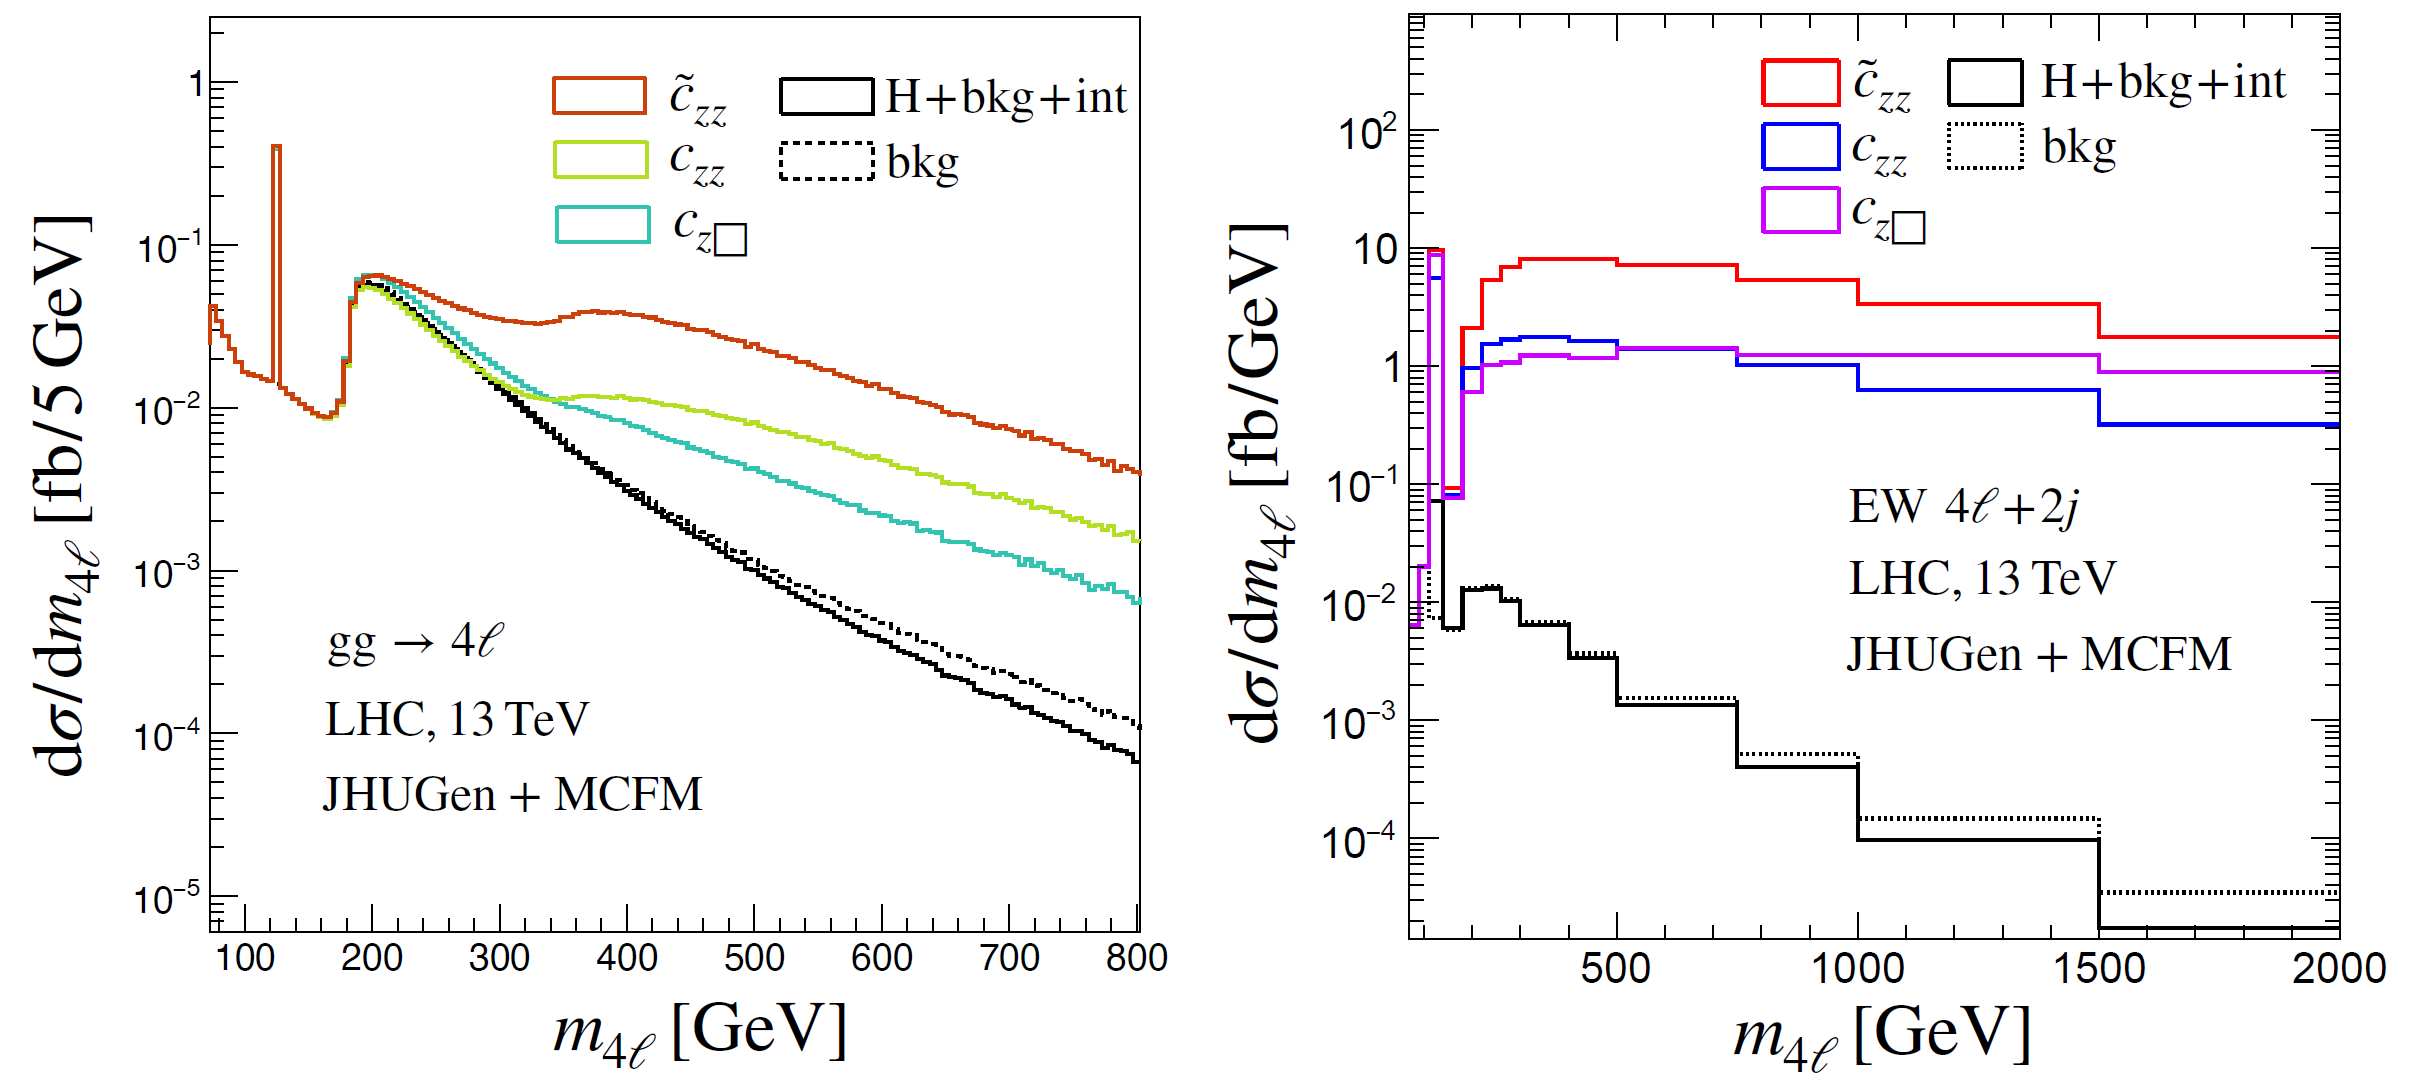
\includegraphics[width=0.8\textwidth,clip] {figures/offshellAC_BSI.png}
\caption{ The four-lepton m4$\ell$ invariant mass distributions for gluon fusion (left) and electroweak production in association with two jets (right) at the LHC with a 13 TeV pp collision energy. The total SM production (“H+bkg+int”) and background-only (“bkg”) components are shown in black. Three operators cz (magenta), czz (blue), and $\tilde{c}$zz (red) are shown
in color, and they are introduced in place of the SM interaction with their strength constrained
to reproduce the SM cross section of the on-shell Higgs boson signal production through gluon
fusion \cite{offshellWGnote}.}
\label{fig:offshellAC_BSI}
\end{figure}

Alternatively, as is done in this analysis, we can reweight these additional samples and leverage the additional statistics to make a more precise measurement. The matrix element likelihood approach (MELA) is used reweight all simulated off-shell events to the SM hypothesis through modified MCFM matrix elements \cite{12077235,10073492}. This eliminates the need for out-of-the-box simulation of additional SM events by utilizing statistics from our BSM simulations instead\footnote{When we incorporate anomalous couplings into future analyses, MELA reweighting will also allow us to create distributions for hypotheses with mixed anomalous contributions to the HVV amplitude. A fact which has already benefited us by significantly reducing the number of uniquely generated samples.}. Furthermore, our analysis improves on past papers \cite{190100174} by including the entire Run2 dataset (spanning years 2016, 2017, and 2018). Table~\ref{tab:samplesDAStable} provides an accounting of the datasets used.

\begin{table}[h]
	\centering
	\resizebox{\textwidth}{!}{%
		\begin{tabular}{|l|l|}
			\hline
			Process         & Dataset Name      \\ \hline
			$gg \rightarrow H \rightarrow ZZ \rightarrow 4\ell$            & /GluGluToHiggs*ToZZTo*\_M125\_GaSM*\_13TeV\_MCFM701\_pythia8/ \\ 
			$q\bar{q} \rightarrow Hqq \rightarrow ZZqq \rightarrow 4\ell qq$    & /VBFToHiggs0*ToZZTo4l\_M125\_GaSM\_13TeV\_JHUGenV730\_MCFM701\_pythia8/ \\ 
			$q\bar{q} \rightarrow W^{\pm}H \rightarrow ZZZ\rightarrow 4\ell + X$    & /VBFToHiggs0*ToZZTo4l\_M125\_GaSM\_13TeV\_JHUGenV730\_MCFM701\_pythia8/ \\ 
			$q\bar{q} \rightarrow ZH \rightarrow ZZZ \rightarrow 4\ell + X$    & /VBFToHiggs0*ToZZTo4l\_M125\_GaSM\_13TeV\_JHUGenV730\_MCFM701\_pythia8/ \\ \hline
			
			$gg \rightarrow H \rightarrow ZZ \rightarrow 4\ell$            & /GluGluHToZZTo4L\_M*\_13TeV\_powheg2\_JHUGenV7011\_pythia8/ \\ 
			$q\bar{q} \rightarrow Hqq \rightarrow ZZqq \rightarrow 4\ell qq$    & /VBF\_HToZZTo4L\_M*\_13TeV\_powheg2\_JHUGenV7011\_pythia8/ \\
			$q\bar{q} \rightarrow W^{+}H \rightarrow ZZZ\rightarrow 4\ell + X$    &  /WplusH\_HToZZTo4L\_M*\_13TeV\_powheg2-minlo-HWJ\_JHUGenV7011\_pythia8/\\ 
			$q\bar{q} \rightarrow W^{-}H \rightarrow ZZZ\rightarrow 4\ell + X$    &  /WminusH\_HToZZTo4L\_M*\_13TeV\_powheg2-minlo-HWJ\_JHUGenV7011\_pythia8/\\ 
			$q\bar{q} \rightarrow ZH \rightarrow ZZZ \rightarrow 4\ell + X$    & /ZH\_HToZZ\_4LFilter\_M*\_13TeV\_powheg2-minlo-HZJ\_JHUGenV7011\_pythia8/ \\ 
			$t\bar{t} \rightarrow H \rightarrow ZZ \rightarrow 4\ell$    & 	/ttH\_HToZZ\_4LFilter\_M*\_13TeV\_powheg2\_JHUGenV7011\_pythia8/ \\ \hline
			
			$q\bar{q} \rightarrow Hqq \rightarrow ZZqq \rightarrow 4\ell qq$    & /VBFToHiggs0PMContinToZZTo*JJ\_M125\_GaSM\_13TeV\_phantom\_pythia8/ \\ 
			$q\bar{q} \rightarrow Hqq \rightarrow ZZqq \rightarrow 4\ell qq$    & /ZZJJTo4L\_EWK\_TuneCP5\_13TeV-madgraph-pythia8/ \\ \hline
			
			$gg \rightarrow H \rightarrow ZZ \rightarrow 4\ell$            & /Higgs0PMToZZTo4L\_M125\_13TeV\_powheg2\_JHUGenV7011\_pythia8/ \\ 
			$q\bar{q} \rightarrow Hqq \rightarrow ZZqq \rightarrow 4\ell qq$    & /VBFHiggs0PMToZZTo4L\_M125\_13TeV\_JHUGenV7011\_pythia8/ \\ 
			$q\bar{q} \rightarrow W^{\pm}H \rightarrow ZZZ\rightarrow 4\ell + X$    & /WHiggs0PMToZZTo4L\_M125\_13TeV\_JHUGenV7011\_pythia8/ \\ 
			$q\bar{q} \rightarrow ZH \rightarrow ZZZ \rightarrow 4\ell + X$    & /ZHiggs0PMToZZ\_4LFilter\_M125\_13TeV\_JHUGenV7011\_pythia8/ \\ \hline
			
			$qq \rightarrow ZZ \rightarrow 4\ell$                           & /ZZTo4L\_13TeV\_powheg\_pythia8/ \\ \hline
		\end{tabular}%
	}
	\caption{Table of datasets used for Higgs production and $ZZ \rightarrow 4\ell$ decay modes.}
	\label{tab:samplesDAStable}
\end{table}

% Here, we have documented inputs used to generate samples that include on-shell events. 
The on-shell samples have already been validated and utilized in CMS analyses~\cite{Sirunyan:2019twz, Sirunyan:2021rug, Sirunyan:2765059}, so we can look to them as a reliable point of comparison for newly generated MC events. There already exist on-shell samples (centered around the 125 GeV Higgs peak) for our dominant production modes generated with POWHEG v2 and JHUGen v7.0.11. We also have as additional samples for electroweak production, on-shell samples generated with JHUGen+JHUGenMELA and off-shell samples of the combined BSI (background+signal+interference) events via Phantom.

These samples are valuable in the validation of the recently produced off-shell samples for gluon fusion and electroweak production, which were generated using JHUGen v7.3.0 interfaced to MCFM v7.0.1 and MCFM v7.0.6. It is important to note here, as we compare on-shell events between all these samples using the cross-section and branching ratio values from Yellow Report (YR) 4, that the off-shell samples share common generator inputs which are not applied to the on-shell samples. These cuts and their associated efficiencies are documented in Table~\ref{tab:geninputtable}.

\begin{table}[h]
	\centering
	\resizebox{\textwidth}{!}{%
		\begin{tabular}{|c|c|c|c|}
			\hline
			Generator           &Sample / Analysis          & Leptons                   & Jets                                \\ \hline
			{JHUGen+MCFM}         &EW off-shell & $pT$ $l_{1,2,3,4} > 3 GeV$, $|\eta$ $l_{1,2,3,4}| < 2.7$ & $pT$ $j_{1,2} >$ 15 GeV, $m_{jj} > $30 GeV, $|\eta$ $j_{1,2}| <$ 6.5, $\Delta R$ $>$ 0.3, $|\Delta\eta$ $j_{1,2}| >$0, $sgn(\eta$ $j_{1}) = \pm sgn(\eta$ $j_{2})$ \\ CLine{2-4} 
			
			&ggH off-shell  & $pT$ $l_{1,2,3,4} > 3 GeV$, $|\eta$ $l_{1,2,3,4}| < 2.7$ & $pT$ $j_{1,2} >$ 15 GeV, $\Delta R$ $>$ 0.4                   \\ \hline
			
			POWHEG+JHUGen                &VBF on-shell  & No specified cuts         & No specified cuts                   \\ CLine{2-4}
			&W$^{-}$H on-shell  & No specified cuts         & No specified cuts                   \\ CLine{2-4}
			&W$^{+}$H on-shell  & No specified cuts         & No specified cuts                   \\ CLine{2-4}
			&ZH on-shell  & No specified cuts         & No specified cuts                   \\ CLine{2-4}
			&ggH on-shell & No specified cuts         & No specified cuts                   \\ \hline
			
			JHUGen+JHUGen           &VBF on-shell         & No specified cuts         & $pT$ $j_{1,2} > 0$ GeV, $\Delta R > 0$ \\ CLine{2-4}
			&WH on-shell         & No specified cuts         & No specified cuts \\ CLine{2-4}
			&ZH on-shell         & No specified cuts         & No specified cuts \\ \hline
			
			Phantom         &EW off-shell (BSI, $4e$) & $pT$ $l_{1,2,3,4} >$ 3 GeV, $|\eta$ $l_{1,2,3,4}| < 2.7$ & $m_{jj} > $30 GeV, $|\eta$ $j_{1,2}| <$ 6.5            \\ CLine{2-4}
			&EW off-shell (BSI, $4\mu$) & $pT$ $l_{1,2,3,4} >$ 3 GeV, $|\eta$ $l_{1,2,3,4}| < 2.7$ & $m_{jj} > $30 GeV, $|\eta$ $j_{1,2}| <$  6.5            \\ CLine{2-4}
			&EW off-shell (BSI, $2e2\mu$) & $pT$ $l_{1,2,3,4} >$ 3 GeV, $|\eta$ $l_{1,2,3,4}| < 2.7$ & $m_{jj} > $30 GeV, $|\eta$ $j_{1,2}| <$ 6.5            \\ \hline
			
		\end{tabular}%
	}
	\caption{Table of generator-level cuts on jets and leptons.}
	\label{tab:geninputtable}
\end{table}



\section{Matrix Element Likelihood Approach}

With up to 13 observables ($\boldsymbol{\Omega}$) describing the \Hboson kinematic distributions in the $2\to 6$ process, visualized in \ref{fig:MELA}, it can be a challenging task to perform an optimal analysis. %in a multidimensional space of observables. 
MELA lets us calculate the matrix elements (ME) for each Higgs boson interaction as a function of its couplings and interacting particles. We can utilize these ME in ratios to change our hypotheses and reweight our Monte-Carlo samples, or treat them as probabilities and construct discriminants to use as observables. 

\begin{figure}[!ht]
\centering
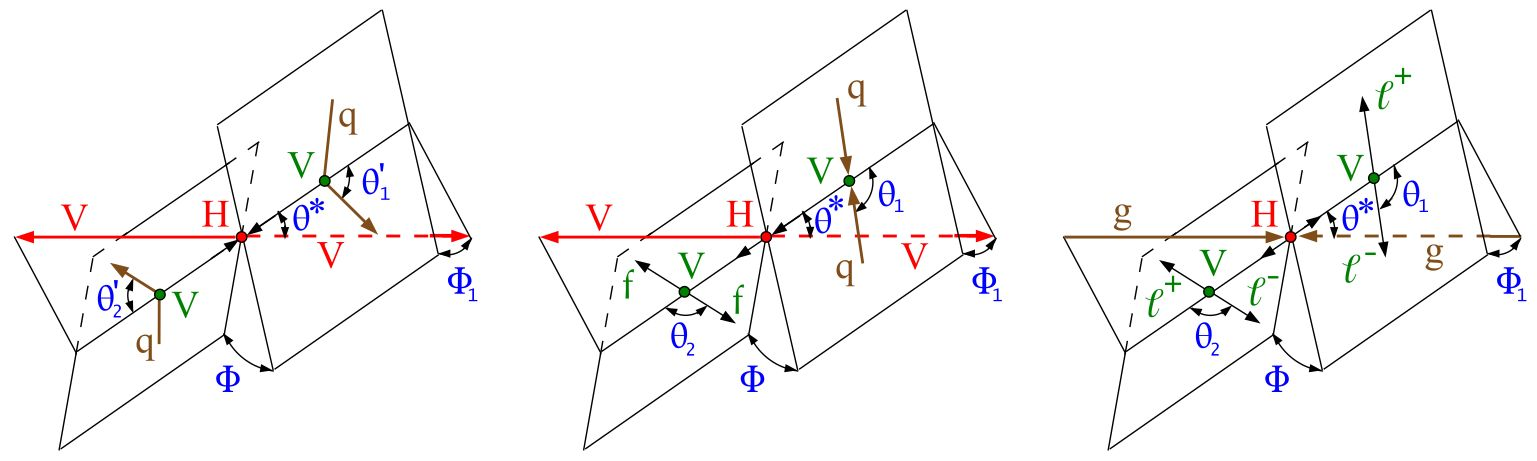
\includegraphics[width=0.8\textwidth,clip] {figures/MELA.jpg}
\caption{Diagrams of relevant kinematic observables in VBF (left), VH (center), and ggH (right) productions of the Higgs boson.}
\label{fig:MELA}
\end{figure}

The MELA approach is designed to reduce the number of observables to the minimum while retaining all essential information. This is a very powerful tool which ensures that our simulations are still based in first principles, but affords us the flexibility to reweight distributions to new hypotheses or combine statistics for greater precision. 

% In order to perform a dedicated study of the particular kinematic topology of HVV, visualized in \ref{fig:MELA}, events are split into several mutually 
% exclusive categories based on the presence of other particles produced in association with the \Hboson candidate~\cite{Sirunyan:2021rug}.
% We use the values of kinematic discriminants, and other selection requirements to perform the categorization. 

% \begin{figure}[!ht]
% \centering
% 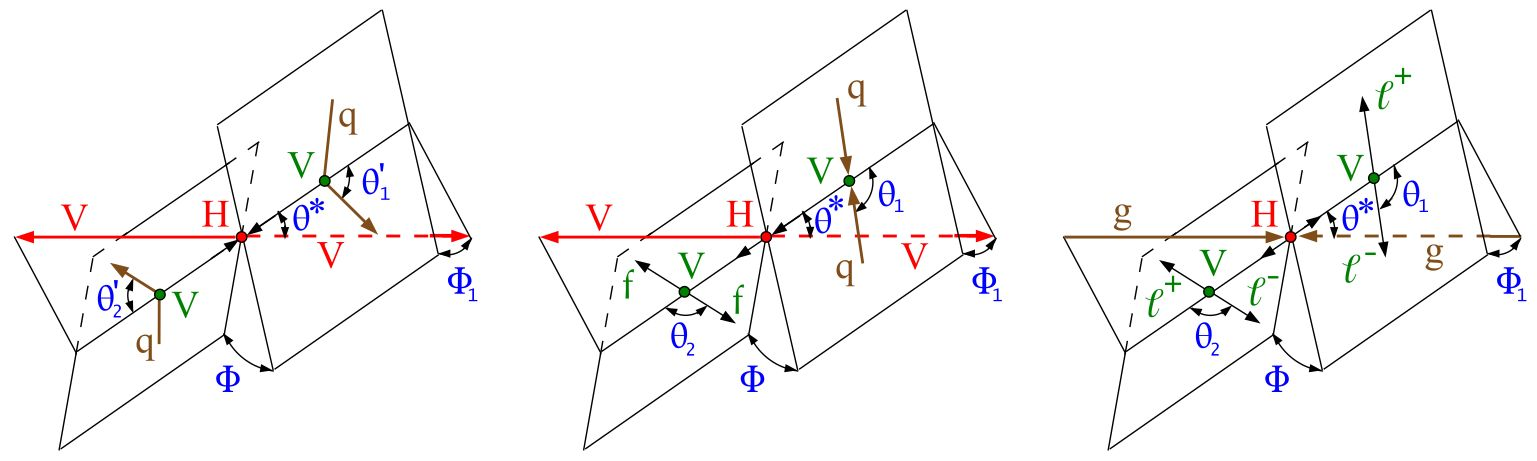
\includegraphics[width=0.8\textwidth,clip] {figures/MELA.jpg}
% \caption{Diagrams of relevant kinematic observables in VBF (left), VH (center), and ggH (right) productions of the Higgs boson.}
% \label{fig:MELA}
% \end{figure}

% The definition of these discriminants can be found in Refs.~\cite{Sirunyan:2017exp,Sirunyan:2017tqd,Sirunyan:2019twz,Sirunyan:2021rug}. 
% They are calculated using the MELA approach while employing the matrix elements at leading order (LO) in quantum chromodynamics (QCD). 

% \begin{equation}
% \mathcal{D}_\mathrm{alt}\left(\boldsymbol{\Omega}\right) = \frac{\mathcal{P}_\text{sig}\left(\boldsymbol{\Omega}\right) }
% {\mathcal{P}_\text{sig}\left(\boldsymbol{\Omega}\right) +\mathcal{P}_\mathrm{alt}\left(\boldsymbol{\Omega}\right) }
% \label{eq:melaD}
% \end{equation}

% \begin{equation}
% \mathcal{D}_\mathrm{int}\left(\boldsymbol{\Omega}\right) =
% \frac{\mathcal{P}_\mathrm{int}\left(\boldsymbol{\Omega}\right) }
% {2 \ \sqrt{{\mathcal{P}_\text{sig}\left(\boldsymbol{\Omega}\right) \ \mathcal{P}_\mathrm{alt}\left(\boldsymbol{\Omega}\right) }}}
% \label{eq:melaDint}
% \end{equation}

% These discriminants use full kinematic information from the \Hboson and from associated jet production and 
% are labeled to indicate a specific topology (2jet) and production mechanism (VBF, WH, ZH), 
% which is discriminated against the dominant gluon fusion process:
% %$\mathcal{D}_\mathrm{1jet}^{VBF}$, 
% $\mathcal{D}_\mathrm{2jet}^{VBF}$, 
% $\mathcal{D}_\mathrm{2jet}^{ZH}$,
% and $\mathcal{D}_\mathrm{2jet}^{WH}$. 
% %The $\mathcal{D}_\mathrm{2jet}$ discriminants are calculated using both SM and anomalous coupling hypotheses, 
% %leading to a set $\mathcal{D}_\mathrm{2jet}^{i}$, all of which 
% %are tested in order to maintain high efficiency of VBF and VH categorization in the presence of anomalous couplings. 
% % Calculation of these discriminants is discussed in more detail later with the presented analysis. 

% % The MELA approach also allows for reweighting between our simulated probability distributions. This has the effect of reducing the number of dedicated 
% % Monte-Carlo simulations required for this analysis, as well as bolstering the available statistics that can be utilized in our templates for Bayesian analysis. 

% \begin{figure}
% \centering
% 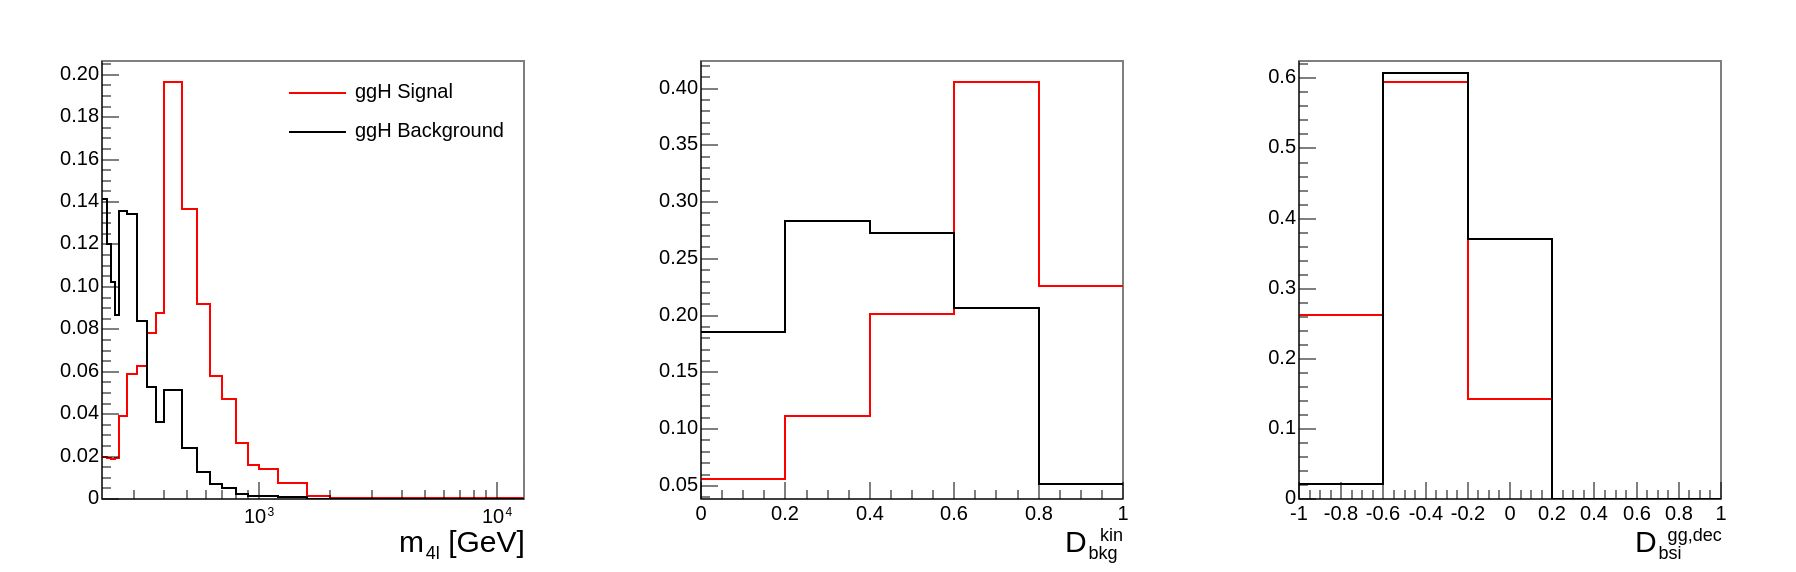
\includegraphics[width=0.8\textwidth,clip] {figures/DiscDists.jpg}
% \caption{}
% \label{fig:DiscDists}
% \end{figure}







\section{Building a $H^{(*)} \rightarrow ZZ^{(*)} \rightarrow 4\ell$ analysis}

\subsection{Reconstructing and selecting events}

% Event reconstruction is based on the particle-flow (PF) algorithm~\cite{Sirunyan:2017ulk}. This algorithm aims to reconstruct and identify each individual particle in an event, with an optimized combination of information from the various elements of the CMS detector. The energy of photons is obtained from the ECAL measurement. The energy of electrons is determined from a combination of the electron momentum at the primary vertex as determined by the tracker, the energy of the corresponding ECAL cluster, and the energy sum of all bremsstrahlung photons spatially compatible with originating from the electron track. The energy of muons is obtained from the curvature of the corresponding track. The energy of charged hadrons is determined from a combination of their momentum measured in the tracker and the matching ECAL and HCAL energy deposits, corrected for the response function of the calorimeters to hadronic showers. Finally, the energy of neutral hadrons is obtained from the corresponding corrected ECAL and HCAL energies.

% Muons with $p_T > 5$ GeV are reconstructed within the geometrical acceptance, corresponding to the region $|\eta|< 2.4$, by combining information from the silicon tracker and the muon systems \cite{MuReco}. The muons are selected among the reconstructed muon track candidates by applying quality requirements on the track in both the muon and silicon tracker systems, and demanding small energy deposits in the calorimeters.

Event reconstruction is based on the particle-flow (PF) algorithm~\cite{Sirunyan:2017ulk}, which endeavors to reconstruct and identify each individual particle in an event by optimally combining information from the various subdetectors of the CMS experiment. Photon energies are determined directly from ECAL measurements. Electron energies are derived from a sophisticated combination of the electron momentum at the primary interaction vertex as measured by the tracker, the energy of the corresponding ECAL cluster, and the integrated energy of all bremsstrahlung photons spatially consistent with emission from the electron trajectory. Muon energies are extracted from the curvature of their tracks in the magnetic field. For charged hadrons, energies are determined by combining their momenta measured in the tracker with the corresponding ECAL and HCAL energy deposits, applying corrections that account for the nonlinear calorimetric response to hadronic showers. The energies of neutral hadrons are obtained from their corrected ECAL and HCAL energy deposits.

Muons with transverse momentum $p_T > 5$ GeV are reconstructed within the geometrical acceptance of $|\eta|< 2.4$ through a comprehensive algorithm that integrates information from both the silicon tracker and the muon detection systems \cite{MuReco}. The selection of muons from among the reconstructed muon track candidates is subject to stringent quality criteria applied to tracks in both the muon chambers and the silicon tracker, complemented by requirements of minimal energy deposition in the calorimeter systems, ensuring high purity in the muon identification. A relative muon isolation variable is defined as

\begin{equation} \label{eqn:pfiso}
  {\mathcal I}^{gm} \equiv \Big( \sum p_T^\text{charged} + \max\big[ 0, \sum p_T^\text{neutral} +
    \sum p_T^{\gamma} - p_T^{\mathrm{PU}} \big] \Big) / p_T,
\end{equation}

where $p_T$ is the muon transverse momentum, and $p_T^{\text{charged}}$, $p_T^\text{neutral}$, and $p_T^\gamma$ are the transverse momentum of charged hadrons, neutral hadrons, and photons, respectively, within a cone radius of $\Delta R=0.3$ around the muon direction at the primary vertex.

Here, $\Delta R(i,j) \equiv \sqrt{\smash[b]{(\eta^i-\eta^j)^{2} + (Hi^i-Hi^j)^{2}}}$, where $Hi$ denotes the azimuthal angle, and indices $\textit{i}$ and $\textit{j}$ refer to the hadron/photon and muon, respectively.
The isolation variable exhibits particular sensitivity to energy deposits from pileup interactions; therefore, a contribution $p_T^{\mathrm{PU}}$ from pileup is subtracted from the isolation parameter, as formulated in Equation~(\ref{eqn:pfiso}). 
This contribution is defined as $p_T^{\mathrm{PU}} = 0.5\sum_{i}p_T^{i,\mathrm{PU}}$, corresponding to 0.5 times the $p_T$ sum of all charged hadrons $i$ not originating from the primary vertex, where the factor of 0.5 accounts for the differing fractions of charged and neutral hadrons~\cite{PUmitigationCMS}. Each muon in the event must satisfy ${\mathcal{I}^{\mu}} < 0.35$.

Photons from final-state radiation are reconstructed using the PF algorithm~\cite{Sirunyan:2017ulk}. Isolated photons satisfying $p_T >2$ GeV, $|\eta| <2.4$, and $\mathcal{I}^{\gamma} < 1.8$ are associated with the nearest lepton (muon or electron) in the event. Photons failing to satisfy the criteria $\Delta R(\gamma,\ell)/(p_T^{\gamma})^2<0.012~\text{GeV}^{-2}$ and $\Delta R(\gamma,\ell) < 0.5$ are excluded from consideration.
When multiple photon candidates fulfill these conditions, the one minimizing $\Delta R(\gamma,\ell)/(p_T^{\gamma})^2$ with respect to the given lepton is retained.
Photons passing these criteria are excluded from the computation of the relative isolation parameter.

Electrons with $p_T>7$ GeV are reconstructed within the geometrical acceptance, defined by the pseudorapidity region $|\eta|<2.5$~\cite{eleReco}. Their identification utilizes a multivariate discriminant incorporating observables sensitive to bremsstrahlung emission along the electron trajectory, the geometric and momentum-energy matching between the electron trajectory and associated ECAL cluster, the electromagnetic shower morphology in the ECAL, and variables discriminating against electrons originating from photon conversions. Electron isolation parameters, defined analogously to those for muons, are integrated into this multivariate discriminant to differentiate between prompt leptons from Z boson decays and those arising from electroweak decays of hadrons within jets. The XGBoost package~\cite{xgboost} is employed for training and optimization of this multivariate discriminant using simulated events that remain independent from all other analysis stages. Separate training procedures are implemented for each of the three data-taking periods \cite{ElectronBDT}. Electrons from photon conversions and muons from in-flight hadronic decays are rejected if the ratio of their three-dimensional impact parameter, computed with respect to the primary vertex position, to its uncertainty exceeds four.

The reconstruction and selection efficiencies for prompt leptons in both data and simulation are evaluated using a tag-and-probe technique~\cite{CMS:2011aa} applied to $Z$ boson event samples. The ratio of efficiencies measured in data to those in simulation is applied as a correction factor to the yields of selected events in the simulated samples.
Furthermore, $Z$ boson events are utilized to calibrate the momentum scale and resolution of electrons and muons as functions of various kinematic variables~\cite{ScaleSmear2, Roch2}.

The selection of Higgs boson candidates requires four prompt and isolated leptons following the aforementioned criteria. 
One lepton must satisfy $p_T>20$ GeV and at least one additional lepton must have $p_T>10$ GeV.
Z boson candidates are constructed from $e^+e^-$ or $\mu^+\mu^-$ pairs with invariant masses in the range 12--120 GeV. 
These dilepton pairs are subsequently combined to form the Higgs boson candidate. 
We denote by $Z_1$ the pair with invariant mass closest to the nominal Z boson mass, 
and by $Z_2$ the remaining pair. Four possible combinations are considered and treated independently: 
$4\mu$, $4e$, $2e2\mu$, and $2\mu2e$, where the mixed-flavor final states are distinguished based on the flavor composition of $Z_{1}$. 
These four combinations exhibit different four-lepton mass resolutions (predominantly determined by whether $Z_{1}$ comprises muons or electrons) 
and contain different amounts of reducible background (largely dependent on whether $Z_{2}$ decays to muons or electrons).
Since none of these flavor-dependent characteristics significantly impacts the off-shell \Hboson analysis, 
all flavor channels are combined in that measurement. 
Signal candidates must satisfy $m_{4\ell} > 70$ GeV. 
When multiple \Hboson candidates can be formed in an event, the one with the highest value of the 
kinematic discriminant $\mathcal{D}_\text{bkg}^\text{kin}$, defined in Section~\ref{sec:categories},
is retained, unless these candidates comprise the same four leptons. 
In the latter case, the candidate whose $Z_1$ invariant mass lies closest to the nominal Z boson mass is selected.

In the off-shell analysis, events undergo further categorization based on jets associated with the \Hboson candidate. 
Jets are clustered using the anti-$k_t$ jet finding algorithm~\cite{Cacciari:2008gp,Cacciari:2011ma} with a distance 
parameter of 0.4. The jet momentum is determined as the vectorial sum of all particle momenta within the jet. 
Jets must satisfy $p_T>30$ GeV and $|\eta|<4.7$ and must be spatially separated
from all selected lepton candidates and any selected final-state radiation photons by requiring 
$\Delta R(\ell/\gamma,\text{jet})>0.4$.
Jets originating from b quark hadronization are identified using the DeepCSV algorithm~\cite{Sirunyan:2017ezt}, which integrates information 
on impact parameter significance, secondary vertex characteristics, and jet kinematic variables. The use of this information is detailed in Section~\ref{sec:categories}.

% Here, $\Delta R(i,j) Equation \refuiv \sqrt{\smash[b]{(\eta^i-\eta^j)^{2} + (Hi^i-Hi^j)^{2}}}$, where $Hi$ is the azimuthal angle, and in this case $\textit{i}$ refers to the hadron or photon, and $\textit{j}$ to the muon.
% Since the isolation variable is particularly sensitive to energy deposits from pileup interactions, a contribution $p_T^{\mathrm{PU}}$ from pileup is subtracted from the isolation parameter, as shown in Equation~(\ref{eqn:pfiso}). 
% It is defined as 0.5 times the $p_T$ sum of all charged hadrons $i$ not originating from the primary vertex $p_T^{\mathrm{PU}} = 0.5\sum_{i}p_T^{i,\mathrm{PU}}$, where the 0.5 factor accounts for the different fraction of charged and neutral hadrons~\cite{PUmitigationCMS}. A requirement of ${\mathcal{I}^{gm}} < 0.35$ is placed on each muon in the event.

% Photons from final-state radiation are reconstructed using the PF algorithm~\cite{Sirunyan:2017ulk}. Isolated photons with $p_T >2$ GeV, $|\eta| <2.4$, and $\mathcal{I}^{\gamma} < 1.8$, are associated with the closest lepton (either muon or electron) in the event. Photons that do not satisfy the requirements $\Delta R(gg,\ell)/(p_T^{\gamma})^2<0.012 GeV^{-2}$ and $\Delta R(gg,\ell) < 0.5$ are discarded.
% If more than one photon candidate fulfils the above conditions, the one with the lowest value of $\Delta R(gg,\ell)/(p_T^{\gamma})^2$ with respect to the given lepton is retained.
% Photons passing the above criteria are excluded from the computation of the relative isolation parameter. 

% Electrons with $p_T>7$ GeV are reconstructed within the geometrical acceptance, corresponding to the pseudorapidity region $|\eta|<2.5$~\cite{eleReco}. They are identified using a multivariate discriminant, which includes observables sensitive to the emission of bremsstrahlung along the electron trajectory, the geometrical and momentum-energy matching between the electron trajectory and the associated cluster in the ECAL, the shape of the electromagnetic shower in the ECAL, and variables that discriminate against electrons originating from photon conversions. The isolation parameter sums for electrons, defined similarly as for muons, are included in the multivariate discriminant. This information is used to discriminate between prompt leptons from Z boson decays and those arising from EW decays of hadrons within jets. The package XGBoost~\cite{xgboost} is used to train and optimize this multivariate discriminant. The training is performed with simulated events that are not used at any other stage of the analysis. Separate trainings are performed for the three different data-taking periods \cite{ElectronBDT}. Electrons from photon conversions and muons from in-flight decays of hadrons are rejected if the ratio of their impact parameter in three dimensions, computed with respect to the primary vertex position, to their uncertainty is greater than four.

% The reconstruction and selection efficiencies for prompt leptons in both data and simulation have been estimated using a tag-and-probe technique~\cite{CMS:2011aa} based on samples of $Z$ boson events. The ratio of the efficiencies measured in data and simulation is used to rescale the yields of selected events in the simulated samples.
% In addition, $Z$ boson events have been used to calibrate the momentum scale and resolution of electrons and muons in bins of different kinematic variables~\cite{ScaleSmear2, Roch2}.

% In the selection of Higgs boson candidates,
% four prompt and isolated leptons are required following the prescription above. 
% One of the leptons must have $p_T>20$ GeV and at least one of the remaining leptons must satisfy $p_T>10$ GeV.
% The Z boson candidates are constructed from $epem$ or $gmpgmm$ pairs whose  invariant mass is in the range 12--120 GeV. 
% The dilepton pairs are then combined to form the Higgs boson candidate. 
% In the following, $Z_1$ denotes the pair with the mass closest to the nominal $Z$ boson mass, 
% while $Z_2$ refers to the remaining one. Four possible combinations are considered and treated separately: 
% 4gm, 4$e$, $2e2gm$, and $2gm2e$, where the mixed-flavor final states are separated based on the decay of $Z_{1}$. 
% The four possible combinations have different four-lepton mass resolutions (largely driven by whether the $Z_{1}$ is formed from 2$gm$ or 2$e$) 
% and different amounts of reducible background (largely driven by whether the $Z_{2}$ decays to 2$\mu$ or 2$e$).
% None of the above differences between the flavor channels affect the off-shell \Hboson analysis 
% and therefore all flavor channels are combined in that measurement. 
% Signal candidates must satisfy $m_{4\ell} > 70$ GeV. 
% If more than one \Hboson candidate can be formed in the event, the one with the highest value of the 
% kinematic discriminant $\mathcal{D}_\text{bkg}^\text{kin}$, defined in Section~\ref{sec:Discriminants},
% is retained, unless these candidates consist of the same four leptons. 
% In this case, the candidate with the $Z_1$ invariant mass closest to the nominal Z boson mass is retained.

% In the off-shell analysis, events are further categorized based on the jets associated with the \Hboson candidate. 
% The jets are clustered using the anti-\kt jet finding algorithm~\cite{Cacciari:2008gp,Cacciari:2011ma} with a distance 
% parameter of 0.4. The jet momentum is determined as the vector sum of all particle momenta in the jet. 
% Jets must satisfy $p_T>30$ GeV and $|\eta|<4.7$ and must be separated
% from all selected lepton candidates and any selected final-state radiation photons by demanding 
% $\Delta R(\ell/\cPgg,{\text{jet}})>0.4$.
% Jets originating from the hadronization of b quarks are identified using the DeepCSV algorithm~\cite{Sirunyan:2017ezt}, which combines information 
% on impact parameter significance, the secondary vertex, and jet kinematic variables. The use of this identification is described in Section~\ref{sec:Discriminants}.

























\subsection{Defining categories and observables} \label{sec:categories}

% With up to 13 observables, $\boldsymbol{\Omega}$, describing the \Hboson kinematic distributions in the $2\to 6$ process,
% it is a challenging task to perform an optimal analysis in a multidimensional space of observables. 
% The MELA approach is designed to reduce the number of observables to the minimum while retaining all essential information. 
% Two types of discriminants were defined for either the production or decay process, and we also combine them into a joint 
% discriminant for the full $2\to 6$ process where relevant.

% \begin{figure}[!ht]
% \centering
% 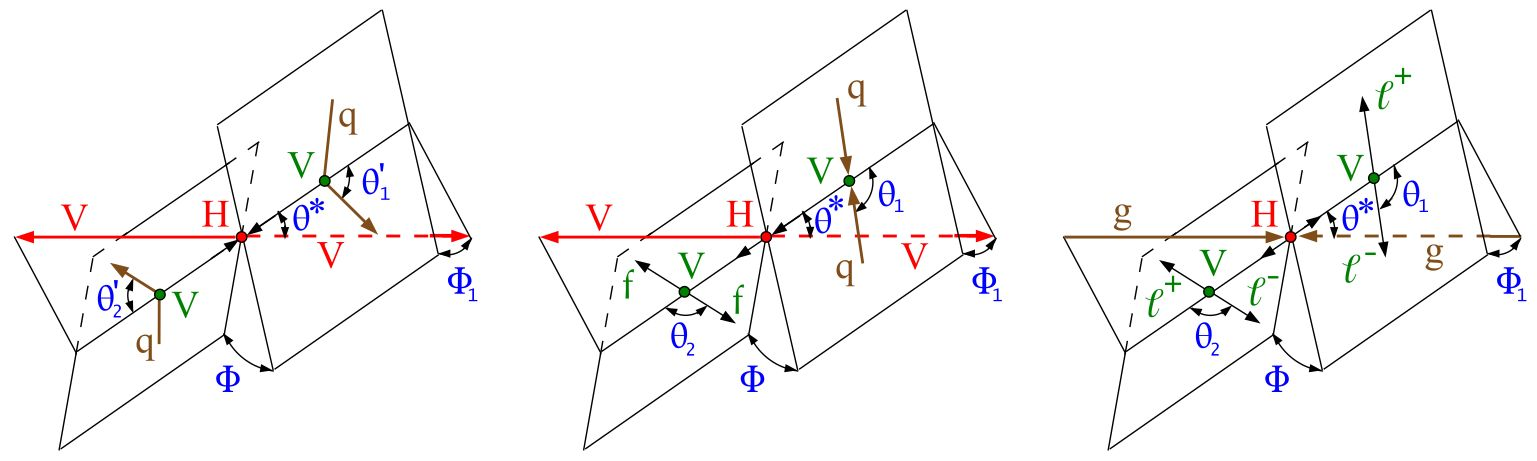
\includegraphics[width=0.8\textwidth,clip] {figures/MELA.jpg}
% \caption{Diagrams of relevant kinematic observables in VBF (left), VH (center), and ggH (right) productions of the Higgs boson.}
% \label{fig:MELA}
% \end{figure}

In order to perform a dedicated study of the particular kinematic topology of HVV, visualized in Figure~\ref{fig:MELA}, events are split into several mutually exclusive categories based on the presence of other particles produced in association with the \Hboson candidate~\cite{Sirunyan:2021rug}. Two types of discriminants are defined for either the production or decay process, which can be combined to describe the full $2\to 6$ process~\cite{Sirunyan:2017exp,Sirunyan:2017tqd,Sirunyan:2019twz,Sirunyan:2021rug}. We use the values of these kinematic discriminants and other selection requirements to perform the categorization. They are calculated using the MELA approach while employing the matrix elements at leading order (LO) in quantum chromodynamics (QCD):
\begin{equation}
	\mathcal{D}_\mathrm{alt}\left(\boldsymbol{\Omega}\right) = \frac{\mathcal{P}_\text{sig}\left(\boldsymbol{\Omega}\right) }
	{\mathcal{P}_\text{sig}\left(\boldsymbol{\Omega}\right) +\mathcal{P}_\mathrm{alt}\left(\boldsymbol{\Omega}\right) }
	\label{eq:melaD}
\end{equation}
\begin{equation}
	\mathcal{D}_\mathrm{int}\left(\boldsymbol{\Omega}\right) =
	\frac{\mathcal{P}_\mathrm{int}\left(\boldsymbol{\Omega}\right) }
	{2 \ \sqrt{{\mathcal{P}_\text{sig}\left(\boldsymbol{\Omega}\right) \ \mathcal{P}_\mathrm{alt}\left(\boldsymbol{\Omega}\right) }}},
	\label{eq:melaDint}
\end{equation}

where the probability of a certain process $\mathcal{P}$ is calculated using the full kinematics characterized
by $\boldsymbol{\Omega}$ for the hypotheses denoted as ``sig'' for a signal model and ``alt'' for an alternative model,
which could be an alternative \Hboson production mechanism (used to categorize events),
background (used to isolate signal), or an alternative \Hboson coupling model (used to measure coupling parameters).
The ``int'' label represents the interference between the two model contributions.
The probabilities $\mathcal{P}$ are calculated from the matrix elements provided by the MELA package and
are normalized to give the same integrated cross sections in the relevant phase space of each process.

These discriminants use full kinematic information from the \Hboson with its associated jets and 
are labeled to indicate a specific topology (2jet) and production mechanism (VBF, WH, ZH), 
which is discriminated against the dominant gluon fusion process:
%$\mathcal{D}_\mathrm{1jet}^{VBF}$, 
$\mathcal{D}_\mathrm{2jet}^{VBF}$, 
$\mathcal{D}_\mathrm{2jet}^{ZH}$,
and $\mathcal{D}_\mathrm{2jet}^{WH}$. 

%The $\mathcal{D}_\mathrm{2jet}$ discriminants are calculated using both SM and anomalous coupling hypotheses, 
%leading to a set $\mathcal{D}_\mathrm{2jet}^{i}$, all of which 
%are tested in order to maintain high efficiency of VBF and VH categorization in the presence of anomalous couplings. 
% Calculation of these discriminants is discussed in more detail later with the presented analysis. 

% The MELA approach also allows for reweighting between our simulated probability distributions. This has the effect of reducing the number of dedicated 
% Monte-Carlo simulations required for this analysis, as well as bolstering the available statistics that can be utilized in our templates for Bayesian analysis. 


The selected events are split into three categories summarized in Table~\ref{tab:categoriesoffshell}: VBF-tagged, VH-tagged, and Untagged.
A set of discriminants $\mathcal{D}_\text{2jet}$ is constructed, following Equation \ref{eq:melaD},
where $\mathcal{P}_\text{sig}$ corresponds to the signal probability for the VBF ($WH$ or $ZH$)
production hypothesis in the VBF-tagged (VH-tagged) category, and $\mathcal{P}_\mathrm{alt}$
corresponds to that of \Hboson production in association with two jets via gluon fusion.
When more than two jets pass the selection criteria, the two jets with the highest $p_T$ are chosen 
for the matrix element calculations. Thereby, the $\mathcal{D}_\text{2jet}$ discriminants separate the 
target production mode of each category from gluon fusion production,
in all cases using only the kinematics of the \Hboson and two associated jets.

\begin{table}[!hbtp]
	\begin{center}
		\begin{tabular}{lccc}
			\hline
			\vspace{-0.2cm}  & & & \\
			~~Category              & VBF-tagged & $VH$-tagged  & Untagged \\
			\vspace{-0.2cm}    & & & \\
			\hline
			%
			\vspace{-0.2cm}  & & & \\
			%
			~~Selection
			& ~~$ \mathcal{D}_{\rm 2jet}^{\rm VBF} >0.5$ 
			& ~~$ \mathcal{D}_{\rm 2jet}^{ZH}$ or $ \mathcal{D}_{\rm 2jet}^{WH}>0.5$
			& ~~Rest of events \\
			%
			&
			& ~~~~
			&   \\
			%
			\vspace{-0.2cm}  & & & \\
			%
			Observables
			&  $m_{4\ell}$, $\mathcal{D}^{{\rm VBF}+{\rm dec}}_{\rm bkg}$, $\mathcal{D}_{\rm bsi}^{{\rm VBF}+{\rm dec}}$
			&  $m_{4\ell}$, $\mathcal{D}^{VH+{\rm dec}}_{\rm bkg}$, $\mathcal{D}_{\rm bsi}^{VH+{\rm dec}}$
			&  $m_{4\ell}$, $\mathcal{D}^{\rm kin}_{\rm bkg}$, $\mathcal{D}_{\rm bsi}^{{\rm gg},{\rm dec}}$  \\
			& & & \\
			% 
			\hline
			%
		\end{tabular}
	\end{center}
    \caption{Summary of the three production categories in the off-shell $m_{4\ell}$ region. All discriminants are calculated with the JHUGen signal and MCFM background matrix elements. The VH interference discriminant in the SM-like analysis hadronic VH-tagged category is defined as the simple average of the ones corresponding to the ZH and WH processes.}
    \label{tab:categoriesoffshell}
\end{table}

In each event category, the observables $\vec{x} = \{ m_{4\ell}, \mathcal{D}_\text{bkg}, \mathcal{D}_\text{int} \}$ are defined following Equations \ref{eq:melaD} and \ref{eq:melaDint},
and as summarized in Table~\ref{tab:categoriesoffshell}. The $\mathcal{D}_\text{bkg}$ observable is calculated with category-dependent methodology. In the untagged category,
$\mathcal{P}_\text{bkg}$ is evaluated for the dominant $q\bar{q}\to4\ell$ background process.  
Both signal and background probability densities incorporate the matrix element probability for a given $m_{4\ell}$ value
as experimentally measured. 

In the VBF-tagged and VH-tagged categories, $\mathcal{P}_\text{bkg}$ and $\mathcal{P}_\text{sig}$ incorporate
not only four-lepton kinematics but also the kinematic properties of the two associated jets.
The $\mathcal{P}_\text{bkg}$ probability density characterizes the combined EW and QCD background processes $4\ell+2$\,jets,
while $\mathcal{P}_\text{sig}$ represents the EW processes VBF and VH. Inclusion of jet kinematics in the
$\mathcal{D}_\text{bkg}$ calculation enhances discrimination of the targeted signal production both against background
and against \Hboson production through gluon fusion.

The third observable, $\mathcal{D}_\text{int}$ defined in Equation \ref{eq:melaDint}, discriminates between the interference
of SM-like \Hboson coupling and background as an alternative model, and is designated
$\mathcal{D}_\text{bsi}$ for the signal-background interference in the off-shell region.
In the untagged category, decay kinematics are utilized in the calculation of $\mathcal{D}_\text{int}$.
In the VBF-tagged and VH-tagged categories, production information incorporating the two associated jets is employed.

% In each category of events, three observables $\vec{x}$ are defined following Equation \ref{eq:melaD} and \ref{eq:melaDint},
% and as summarized in Table~\ref{tab:categoriesoffshell}, $\vec{x} = \{ m_{4\ell}, \Dbkg, \Dint \}$.
% The \Dbkg observable is calculated differently in the three tagged categories. In the untagged category,
% $\mathcal{P}_\text{bkg}$ is calculated for the dominant $q\bar{q}\to4\ell$ background process.  
% The signal and background probabilities include the matrix element probability for a given $m_{4\ell}$ mass,
% as measured in experiment. 
% In the VBF-tagged and VH-tagged categories, $\mathcal{P}_\text{bkg}$ and $\mathcal{P}_\text{sig}$ include
% four-lepton kinematics and kinematic information of the two associated jets.
% The $\mathcal{P}_\text{bkg}$ probability density represents the EW and QCD background processes $4\ell+2$\,jets,
% while $\mathcal{P}_\text{sig}$ represents EW processes VBF and VH. It was found that jet kinematics in the
% \Dbkg calculation improves separation of the targeted signal production both against background
% and against the \Hboson gluon fusion production.

% The third observable, \Dint defined in Equation \ref{eq:melaDint}, separates the interference
% of the SM-like \Hboson coupling and background as an alternative model, and is called
% \Dbsi for the signal-background interference in the off-shell region.
% In the untagged category, decay information is used in the calculation of \Dint.
% In the VBF-tagged and VH-tagged categories, production information with the two associated jets is used.

\begin{figure}[!ht]
\centering
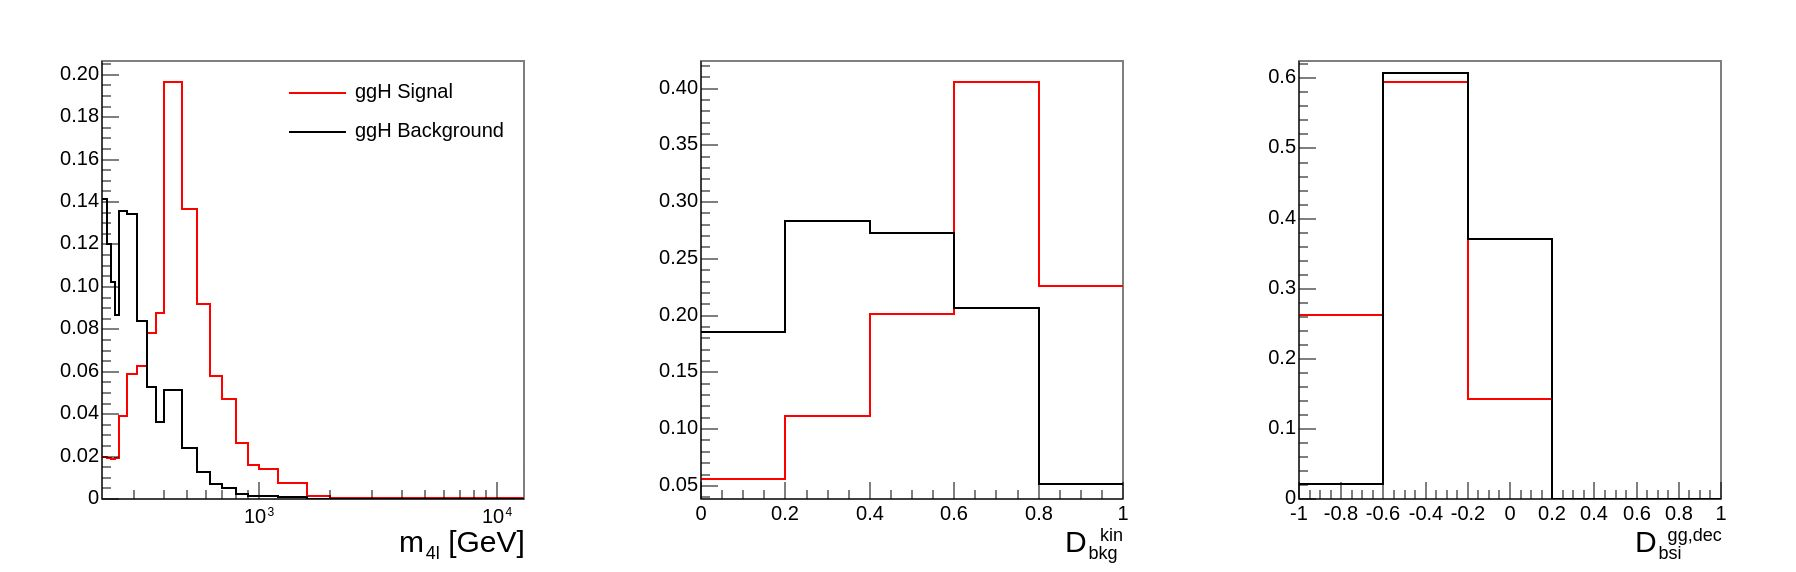
\includegraphics[width=0.8\textwidth,clip] {figures/DiscDists.jpg}
\caption{}
\label{fig:DiscDists}
\end{figure}

The gluon fusion cross section is computed utilizing the highest-order QCD and electroweak (EW) expansions available for inclusive $ZZ$ production~\cite{deFlorian:2016spz}. 
However, event categorization relies on the modeling of associated jets through PYTHIA's parton showering and hadronization algorithms, which necessitates proper matching to the underlying hard-scattering process. Off-shell gluon fusion production is generated at leading order (LO) without associated jets at the matrix element level, implying that all reconstructed jets originate from PYTHIA's modeling. 
The parton showering and hadronization processes require specification of the hadronization scale, which is typically dependent on the characteristic energy scale of the process—set to $m_{4\ell}$ in the case of $gg\to 4\ell$.

For EW production mechanisms, the inclusive production cross section of $ZZ$ with two associated jets is similarly calculated using the highest-order QCD and EW expansions available~\cite{deFlorian:2016spz}. 
In contrast to gluon fusion, two hard jets—typically the leading jets in the event—are generated intrinsically at the matrix element level in the LO simulation. 
These jets correspond to either the forward-backward jets characteristic of vector boson fusion (VBF), or to the hadronic decay products of an associated W or Z boson. 
Consequently, the dependence on PYTHIA's parton shower and hadronization algorithms, and their matching to the hard-scattering production, is substantially reduced for these EW processes.

The categorization efficiency for simulated ggH and EW \Hboson production can be validated through comparison with alternative POWHEG and MINLO simulations. 
The POWHEG samples are generated across a broad range of off-shell \Hboson masses at next-to-leading order (NLO) in QCD, with one jet generated at the matrix element level and additional jets simulated through PYTHIA matching. 
The MINLO simulation of ggH production is performed for \Hboson masses of 125 and $300$ GeV at NLO in QCD, with two jets generated at the matrix element level and additional jets modeled via PYTHIA matching.

While JHUGen categorization efficiencies are consistent with those from POWHEG and MINLO within the uncertainties associated with the QCD scale implementation in PYTHIA,
the ggH process exhibits deviations in central values and corresponding uncertainties of up to 20\% in the signal-dominated $m_{4\ell}$ range of 300--500 GeV, with category-dependent variations. 
For EW processes, categorization efficiencies typically agree within 5--10\% between methodologies. 
We implement a correction procedure whereby the categorization efficiency as a function of $m_{4\ell}$ is adjusted to match that of the SM signal derived from POWHEG samples, with the assumption that this correction applies equally to background and interference contributions. 
This procedure ensures conservation of the total event yield across all three categories at each $m_{4\ell}$ value.

The simulation of the $\vec{x}$ observables enumerated in Table~\ref{tab:categoriesoffshell} remains unaffected by jet modeling in the Untagged category. Furthermore, the modeling of observables in jet-tagged categories for EW processes demonstrates remarkable consistency between direct MCFM + JHUGen samples and reweighted POWHEG + JHUGen implementations. 
However, jet modeling in jet-tagged categories for the ggH process significantly impacts the parametrization of probability distributions. Therefore, within these two jet-tagged categories, the gluon fusion process is implemented through reweighted POWHEG + JHUGen simulation, which provides more precise parton shower matching and consequently superior modeling of associated jet activity. In this framework, samples are reweighted according to the appropriate theoretical model using the MELA package.

% The gluon fusion cross section is calculated using the highest order QCD and EW expansions available 
% to simulate inclusive $ZZ$ production~\cite{deFlorian:2016spz}.
% However, event categorization depends on modeling associated jets through PYTHIA's parton showering and hadronization, 
% which involves matching these processes to the hard-scattering production. Off-shell gluon fusion production is generated at LO 
% with no associated jets at the matrix element level, and therefore all jets come from PYTHIA. 
% The parton showering and hadronization requires setting the hadronization scale, which can depend on the energy scale 
% in the process. In the case of the $gg\to 4\ell$ process, the energy scale is set at $m_{4\ell}$.

% The EW cross section for the inclusive production of $ZZ$ and two associated jets is also calculated to the highest order 
% QCD and EW expansion available~\cite{deFlorian:2016spz}. 
% Contrary to the gluon fusion process, two hard jets, which are typically the leading 
% jets in the process, are already generated at the matrix element level in the LO simulation. 
% These are the two associated jets in the VBF process, or 
% the two jets from the hadronic decay of the associated W or Z boson. 
% Therefore, the dependence on the PYTHIA parton shower and hadronization 
% and its matching to the hard-scattering production is much weaker for these EW processes. 

% The categorization efficiency of simulated ggH and EW \Hboson production can be checked using alternative POWHEG and MINLO simulations. 
% The POWHEG samples are generated for a wide range of off-shell \Hboson masses at NLO in QCD, 
% with one jet generated at the matrix element, and using PYTHIA matching to simulate additional jets. 
% The MINLO simulation of ggH production is done for \Hboson masses of 125 and $300$ GeV at NLO in QCD, 
% with two jets generated at the matrix element level, and PYTHIA matching for additional jets.
% While the JHUGen categorization efficiencies agree with those using POWHEG and MINLO 
% within the uncertainties of the QCD scale used in PYTHIA,
% for the ggH process the deviations of the central values and the corresponding uncertainties 
% are up to 20\% in the signal-dominated $m_{4\ell}$ range 300--500 GeV, depending on the category. 
% In the EW process, categorization efficiencies from the two approaches typically agree within 5--10\%. 
% In all cases, we adjust the categorization efficiency as a function of $m_{4\ell}$ to match that for the SM signal 
% obtained from the POWHEG samples, and assume the same behavior for 
% the background and interference contributions. 
% This correction procedure ensures that the total event yield, summed over the three categories,
% is unchanged at each value of $m_{4\ell}$.

% Simulation of the $\vec{x}$ observables listed in Table~\ref{tab:categoriesoffshell}
% is not affected by the jet modeling in the Untagged category. It is also found that the modeling
% of the observables in the jet-tagged categories is nearly the same in the EW process, when 
% compared between the direct MCFM + JHUGen samples and reweighted POWHEG + JHUGen. 
% However, the modeling of jets in the jet-tagged categories for the ggH process does impact 
% the parametrization of the probability distributions. Therefore, within these two jet-tagged categories, 
% the gluon fusion process is incorporated through the reweighted POWHEG + JHUGen simulation. 
% This approach allows a more precise matching with the parton shower, thereby 
% better describing the associated jet activity. In this case, the samples are reweighted for the appropriate 
% model using the MELA package.

\subsection{Parameterizing the off-shell Higgs boson}

In the off-shell region, the probability density follows Eqs.~(\ref{eq:resonant}) and~(\ref{eq:ponshell}) closely,
with the additional contribution of the interference (``int'') between the signal and background amplitudes,
as well as a cross-feed (``cross'') component discussed below. It is parametrized as 
\begin{equation}\label{eq:poffshell}
    \mathcal{P}_{jk}(\vec{x};\vec{\xi}_{jk},\vec\zeta) =
    \frac{\mu_j \Gamma_H}{\Gamma_0}\mathcal{P}_{jk}^\text{sig} ( \vec{x};\vec{\xi}_{jk})
    + \sqrt{\frac{\mu_j \Gamma_H}{\Gamma_0}}\mathcal{P}_{jk}^\mathrm{int} ( \vec{x};\vec{\xi}_{jk})
    + \mu_j\mathcal{P}_{jk}^\text{cross} (\vec{x};\vec{\xi}_{jk})
    + \mathcal{P}_{jk}^\text{bkg} ( \vec{x};\vec{\xi}_{jk}),
\end{equation}
where $\Gamma_0$ is the reference value of the \Hboson width (not necessarily its SM value)
used in simulation. Otherwise, the definition of the terms is the same as in Equation~(\ref{eq:ponshell}). 
In the off-shell width analysis, there are two production modes, $j$ (gluon fusion and EW, which includes both VBF and VH), 
and three jet-tagged categories, $k$. All lepton flavors and data periods are combined in this analysis.
The contributions from ttH, bbH, and tqH are expected to be negligible in the off-shell region.

The $\mathcal{P}_{jk}^{\text{sig}}$, $\mathcal{P}_{jk}^{\text{int}}$, $\mathcal{P}_{jk}^{\text{cross}}$, and $\mathcal{P}_{jk}^\text{bkg}$ probability densities
are normalized to the expected number of events, and are implemented as binned histograms (templates)
of the observables $\vec{x}$ listed in Table~\ref{tab:categoriesoffshell}.
These templates are obtained as weighted linear combinations of existing simulated signal or background samples.

\subsubsection{Cross-feed effect}

The off-shell region includes all events with $m_{4\ell}$ greater than $220$ GeV. 
Other processes can mimic off-shell \Hboson production and decay to four leptons in this region. 
Specifically, we study on-shell signal events in which the \Hboson decays 
to $2\ell +X$, and $X$ contains further leptons that allow the event to pass the four-lepton selections. 
The dominant on-shell \Hboson process that can contaminate the off-shell region is $Z(\ell\ell)H(2\ell+X)$, called $ZH$ cross-feed. 

The $ZH$ cross-feed contribution is estimated using on-shell 
$ZH$ samples with $H \to WW$ and $ZZ$ decays, 
where both hadronic and leptonic decay of the Z bosons is allowed. 
The dominant contributions come from the $H \to 2\ell 2gn$ and $2\ell 2\Pq$ final states
produced in association with $Z\to 2\ell$. 
To prevent double counting, on-shell cross-feed events are eliminated from the off-shell simulated samples.

\subsection{Parameterizing the on-shell Higgs boson}

The probability density for the on-shell region includes both signal and background contributions.  It is normalized to the total event yield for each process $j$ and category $k$, and can be written as
\begin{equation}
  \mathcal{P}_{jk}(\vec{x};\vec{\xi}_{jk},\vec\zeta) = 
  \mu_j\mathcal{P}_{jk}^\text{sig} (\vec{x};\vec{\xi}_{jk},\vec\zeta) +
  \mathcal{P}_{jk}^\text{bkg}(\vec{x};\vec{\xi}_{jk}),
  \label{eq:ponshell}
\end{equation}
where $\vec\zeta$ are the unconstrained parameters of interest,
including the signal strength $\mu_j$ defined as the ratio of the signal yield to the SM expectation,
$\vec{\xi}_{jk}$ are the constrained nuisance parameters for a particular parametrization,
and $\vec{x}$ are the observables.


\section{Measurement of Higgs boson properties}

\subsection{Off-shell Signal Strength}

\subsection{Higgs boson Width}

We perform an extended binned maximum likelihood fit to the on- and off-shell events split in several categories. 
The final measurements of $m_H$, $\Gamma_H$, and $\mu_{j}$ are conducted using the
 CMS statistical analysis tool \textsc{Combine}~\cite{CMS:2024onh}. 

The extended likelihood function is constructed using the probability densities in
Eqs.~(\ref{eq:ponshell}) and~(\ref{eq:poffshell}), with each event characterized by the discrete category $k$ and typically three 
observables $\vec{x}$. The likelihood $\mathcal{L}$ is maximized with respect to the nuisance parameters $\vec{\xi}_{jk}$ describing
the systematic uncertainties and the signal strength parameter $\mu$ (total signal strength), 
or $\mu_F$ (signal strength for ggH) and $\mu_V$ (signal strength for the EW processes). The allowed 68 and 95\% CL 
intervals are defined using the profile likelihood function, $-2\Delta\ln\mathcal{L} = 1.00$ and $3.84$, 
respectively, for which exact coverage is expected in the asymptotic limit~\cite{Wilks:1938dza}.

Constraints on $\Gamma_H$ are set by simultaneously fitting $H\toZZ\to4\ell$ events from the on- and off-shell regions. 
The on-shell region corresponds to Scheme 2 in Ref.~\cite{CMS:2021nnc}, 
where six mutually exclusive event categories are defined and anomalous interactions are constrained to zero. 
It determines two signal strengths, $\mu_j$ in Eqs.~(\ref{eq:ponshell}) and~(\ref{eq:poffshell}), 
labeled as $\mu^\text{on-shell}_{F}$ and $\mu^\text{on-shell}_{V}$, 
which correspond to production mechanisms driven by fermion and vector boson couplings of
the \Hboson, respectively. 
The \Hboson mass is constrained to $m_H$=125.38 GeV \cite{Sirunyan:2020xwk} in this fit. 
The observed and expected constraints on the \Hboson width are shown in Table~\ref{table:widthoffshellcomb}.
The likelihood scan of $\Gamma_H$ using the asymptotic approximation method is shown in Fig.~\ref{fig:widthscan}. 
This measurement excludes the scenario of no off-shell \Hboson production with a CL corresponding 
to 3.0 standard deviations (average expected 1.4).

\begin{table*}[!htb]
    \centering
    % \renewcommand{\arraystretch}{1.25}
    \begin{tabular}{lll}
        Channel     & Observed $\Gamma_H$ (MeV)        &  Expected $\Gamma_H$ (MeV)  \\
        \hline
        $4\ell$ on- and off-shell    & $2.9^{+2.3}_{-1.7} \ [0.3,7.9]$ & $4.1\pm 4.0 \ [<11.5 ]$ \\
        $4\ell$ on- and off-shell  + $2\ell2\nu$ off-shell  & $3.0^{+ 2.0 }_{- 1.5 }  \ [0.6, 7.3]$ & $4.1\pm3.5 \ [0.1,10.5]$ \\
    \end{tabular}
    \caption{Summary of the total Higgs boson width $\Gamma_H$ measurement, showing the 68\%~CL (central values with uncertainties)
    and 95\%~CL (in square brackets) intervals for the $H\toZZ\to4\ell$ channel alone and in combination with the 
    off-shell $H\to ZZ\to2\ell2\nu$ channel.}
    \label{table:widthoffshellcomb}
\end{table*}

\begin{figure}[!htb]
    \centering
    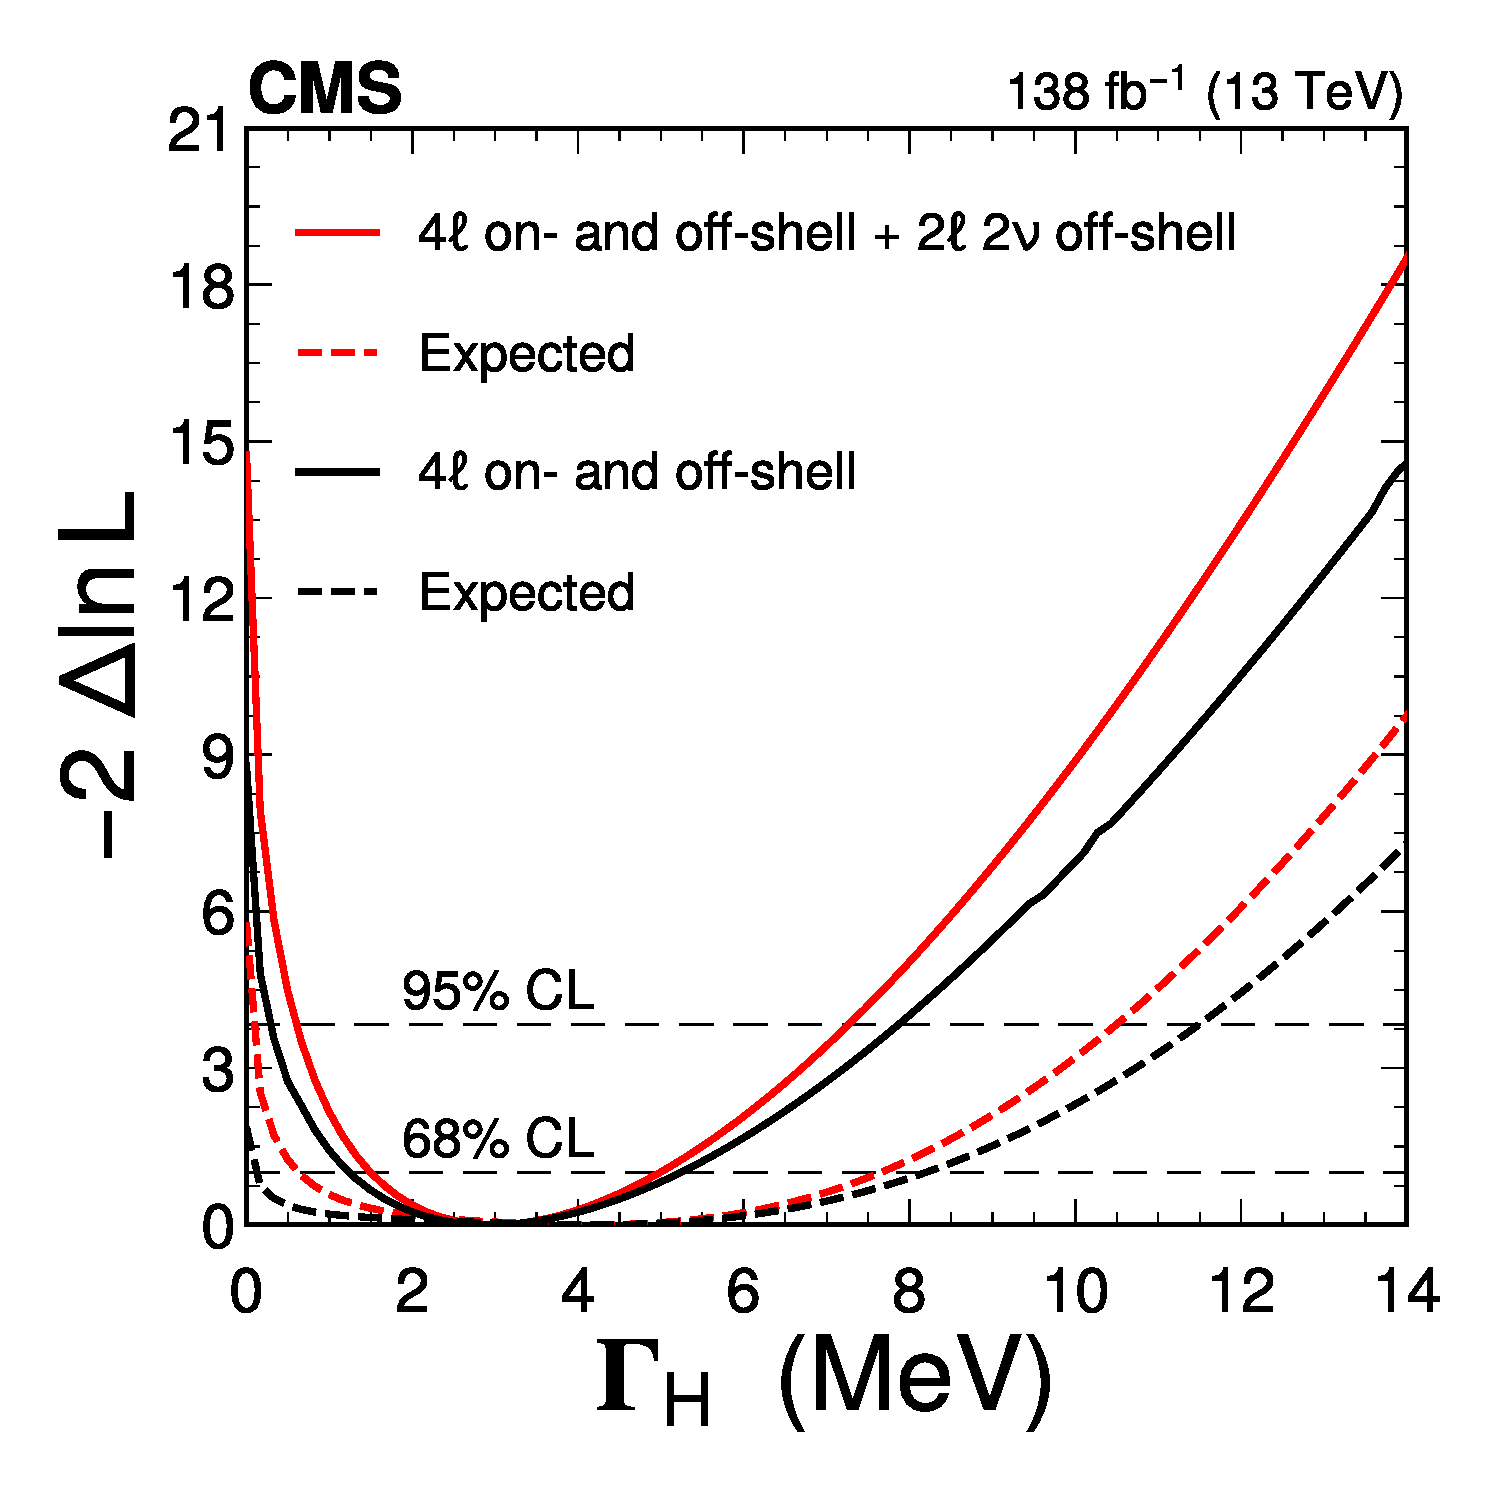
\includegraphics[width=0.45\textwidth]{Figure_011.pdf}  
    \caption{
        Observed (solid) and expected (dashed) profile likelihood projections from the \Hboson width fit using on- and off-shell production from this analysis. The analysis of the off-shell $H\to ZZ\to4\ell$ channel combined with the on-shell $H\toZZ\to4\ell$ channel~\cite{CMS:2021nnc} is shown in black. The full combination of $H\toZZ\to4\ell$ with the off-shell $H\toZZ\to2\ell2\nu$~\cite{CMS:2022ley} is given in red. The black horizontal dashed lines show the 68 and 95\% CL values. }
    \label{fig:widthscan} 
\end{figure}

The observed limits on $\Gamma_H$ are stronger than the average expected values from simulation. 
This is supported by our template plots, where the number of observed events in the 
sensitive region of $m_{4\ell}>340$ GeV and $\Dbkg > 0.6$ in the Untagged category is below the expected value, but still consistent with it. 
The smaller number of events in this region favors the hypothesis of negative interference between the signal and background 
contributions, which dominates over the pure signal contributions for $\Gamma_H$ values near the SM value. 
Therefore, large and very small values of $\Gamma_H$ are disfavored.



\subsection{Kappa Framework}

\subsection{Other measurements}

\subsubsection{Overall Signal Strength}

\subsubsection{Higgs Mass}

Compared to the previous CMS on-shell \Hboson measurement in this channel~\cite{Sirunyan:2017exp}, 
the statistical and systematic uncertainties affecting $m_{H}$ have been reduced by including the beam spot in a refit of the muon tracks; adopting an improved event categorization procedure; and performing a detailed study of the lepton momentum scale and resolution.

The \Hboson mass is measured, using on-shell production, by fitting the $m_{4\ell}$ distribution in the mass range $105< m_{4\ell} < 140$ GeV, using different likelihood models. % as described in Section~\ref{onshellmodel}.
The results have been determined using the CMS statistical analysis tool COMBINE~\cite{CMS:2024onh}, 
which is based on the \textsc{RooFit}~\cite{Verkerke:2003ir} and \textsc{RooStats}~\cite{Moneta:2010pm} frameworks.\\
Table~\ref{table:Mass1Dresults} shows
the mass measurements obtained from the 1D approach, where no further assumptions have been made.
In comparison to the 1D model, the 1D$^{'}_\text{BS}$ model reduces the uncertainty by about 15\%.
Implementing the $\delta m_{4\ell} / m_{4\ell}$ categorization then gives the $\mathcal{N}$--1D$'_\text{BS}$ model, which leads to an additional 10\% improvement. 
Finally, using the \Dkinbkg discriminant to reduce the background produces the $\mathcal{N}$--2D$'_\text{BS}$ model with another 4\% improvement. 
Table~\ref{table:Mass_results} shows the resulting $m_{4\ell}$ measurements using this last model. 
All the measured $m_{4\ell}$ values from the different fits are statistically compatible, given their uncertainties and correlations.
Figure~\ref{MassLikelihoodScan} displays the observed 1D likelihood scans as functions of $m_H$, from the fits for the different $4\ell$ categories and combined.
Combining all the $m_{4\ell}$ final states and data-taking years, our final result is 
$m_H = 125.04~\pm~0.11$ (stat)$~\pm~0.05$ (syst) = $125.04~\pm~0.12$ GeV.
The largest systematic uncertainty is from the lepton momentum scale and equals 0.03 and 0.04  GeV for final states with muons and electrons, respectively.

\begin{table*}[!htb]	
  \centering
  \topcaption{
    Best fit values for the mass of the \Hboson measured in the inclusive 4$\ell$ final state and separately for different flavor categories using the 1D approach.
    Uncertainties are separated into statistical and systematic uncertainties.
    Expected uncertainties are also given assuming $m_{H} = 125.38$ GeV \cite{Sirunyan:2020xwk}.
  }
  \renewcommand{\arraystretch}{1.6}
    \begin{tabular}{lcc}
      $4\ell$ category & Observed ($\pm$stat$\pm$syst) (GeV) & Expected uncertainty ($\pm$stat$\pm$syst)  (GeV) \\
      \hline
      Inclusive &	$124.98 \pm 0.14 \pm0.05$ & $ \pm 0.14 \pm 0.05$ \\
      $4\mu$ &	$124.87 \pm 0.17\pm0.04$ & $\pm 0.18 \pm 0.04$ \\
      $2\mu2e$ &	$125.32^{+0.36}_{-0.37}\pm0.10$ & $^{+0.34+0.09}_{-0.34-0.10}$ \\
      $2e2\mu$ &        $125.23^{+0.36+0.09}_{-0.35-0.11}$ & $^{+0.35+0.09}_{-0.35-0.10}$ \\
      ${4e}$ &    $124.94^{+0.68}_{-0.71} \pm 0.20$ & $^{+0.51+0.18}_{-0.51-0.20}$ \\
  \end{tabular}
  \label{table:Mass1Dresults}
\end{table*}

\begin{table*}[!htb]	
  \centering
  \topcaption{Best fit values for the mass of the \Hboson measured in the inclusive 4$\ell$ final state and separately for different flavor categories, using the final fit configuration ($\mathcal{N}$--2D'$_\text{BS}$).  Uncertainties are separated into statistical and systematic uncertainties. Expected uncertainties are also given assuming $m_{H} = 125.38$ GeV \cite{Sirunyan:2020xwk}.}
  \renewcommand{\arraystretch}{1.6}
    \begin{tabular}{lccc}
      $4\ell$ category & Observed ($\pm$stat$\pm$syst) (GeV) & Expected uncertainty ($\pm$stat$\pm$syst) (GeV)  \\
      \hline
      Inclusive  & $125.04\pm0.11 \pm 0.05$	&	 $\pm 0.11\pm  0.05$ \\
      $4\mu$ & $124.90 \pm 0.14 \pm 0.05$	&	$\pm 0.14\pm  0.04$ \\
      $2e2\mu$ &        $125.50^{+0.25}_{-0.24}\pm0.10$      &       $\pm0.24\pm0.10$ \\
      $2\mu2e$ &        $125.20^{+0.27+0.11}_{-0.26-0.07}$     &        $\pm0.27\pm0.10$ \\
      $4e$ &	$124.70^{+0.49}_{-0.47}\pm0.20$     &	$\pm0.38\pm0.20$ \\ 
  \end{tabular}
  \label{table:Mass_results}
\end{table*}

As a check on the analysis technique and the systematic uncertainty from this method, the 
1D$^{'}_\text{BS}$ model is applied to $Z \to 4\ell$ events in the $m_{4\ell}$ range 70--105  GeV. The signal shape is obtained using a convolution of a Breit--Wigner function and a double-sided Crystal Ball function.
The fitted values of $m_Z$ in different subchannels are $m_Z^{4\mu} = 91.02 \pm 0.14$ GeV, $m_Z^{4e} = 91.18 \pm 0.45$ GeV, $m_Z^{2e2\mu} = 91.40 \pm 0.29$ GeV, and $m_Z^{2\mu2e} = 91.40 \pm 0.37$ GeV, leading to a combined value of $m_Z = 91.17 \pm 0.12$ GeV, consistent with the world-average Z boson mass~\cite{Agashe:2014kda} and with the uncertainty in agreement with the expected value of $\pm~0.12$ GeV from simulation.

The results from this analysis are combined with those extracted using data recorded with the  
CMS detector during Run1 at $\sqrt{s}= 7$ and 8 TeV~\cite{Chatrchyan:2013mxa}. 
Since this analysis uses an improved method to extract the systematic uncertainties affecting lepton momentum, 
the lepton energy scales and resolution uncertainties are considered uncorrelated between the two runs. The combined observed result from
both data-taking periods is $m_H$ = 125.08 $\pm$ 0.12 GeV = 125.08 $\pm$ 0.10\stat $\pm$ 0.05\syst GeV.
The corresponding expected statistical and systematic uncertainties are $\pm$0.10 and $\pm$0.05 GeV, respectively. 
Figure~\ref{Run1Run2_scan} presents a summary of the \Hboson mass measurements by the CMS Collaboration in the four-lepton decay channel.
\begin{figure}[!htb]
  \centering
  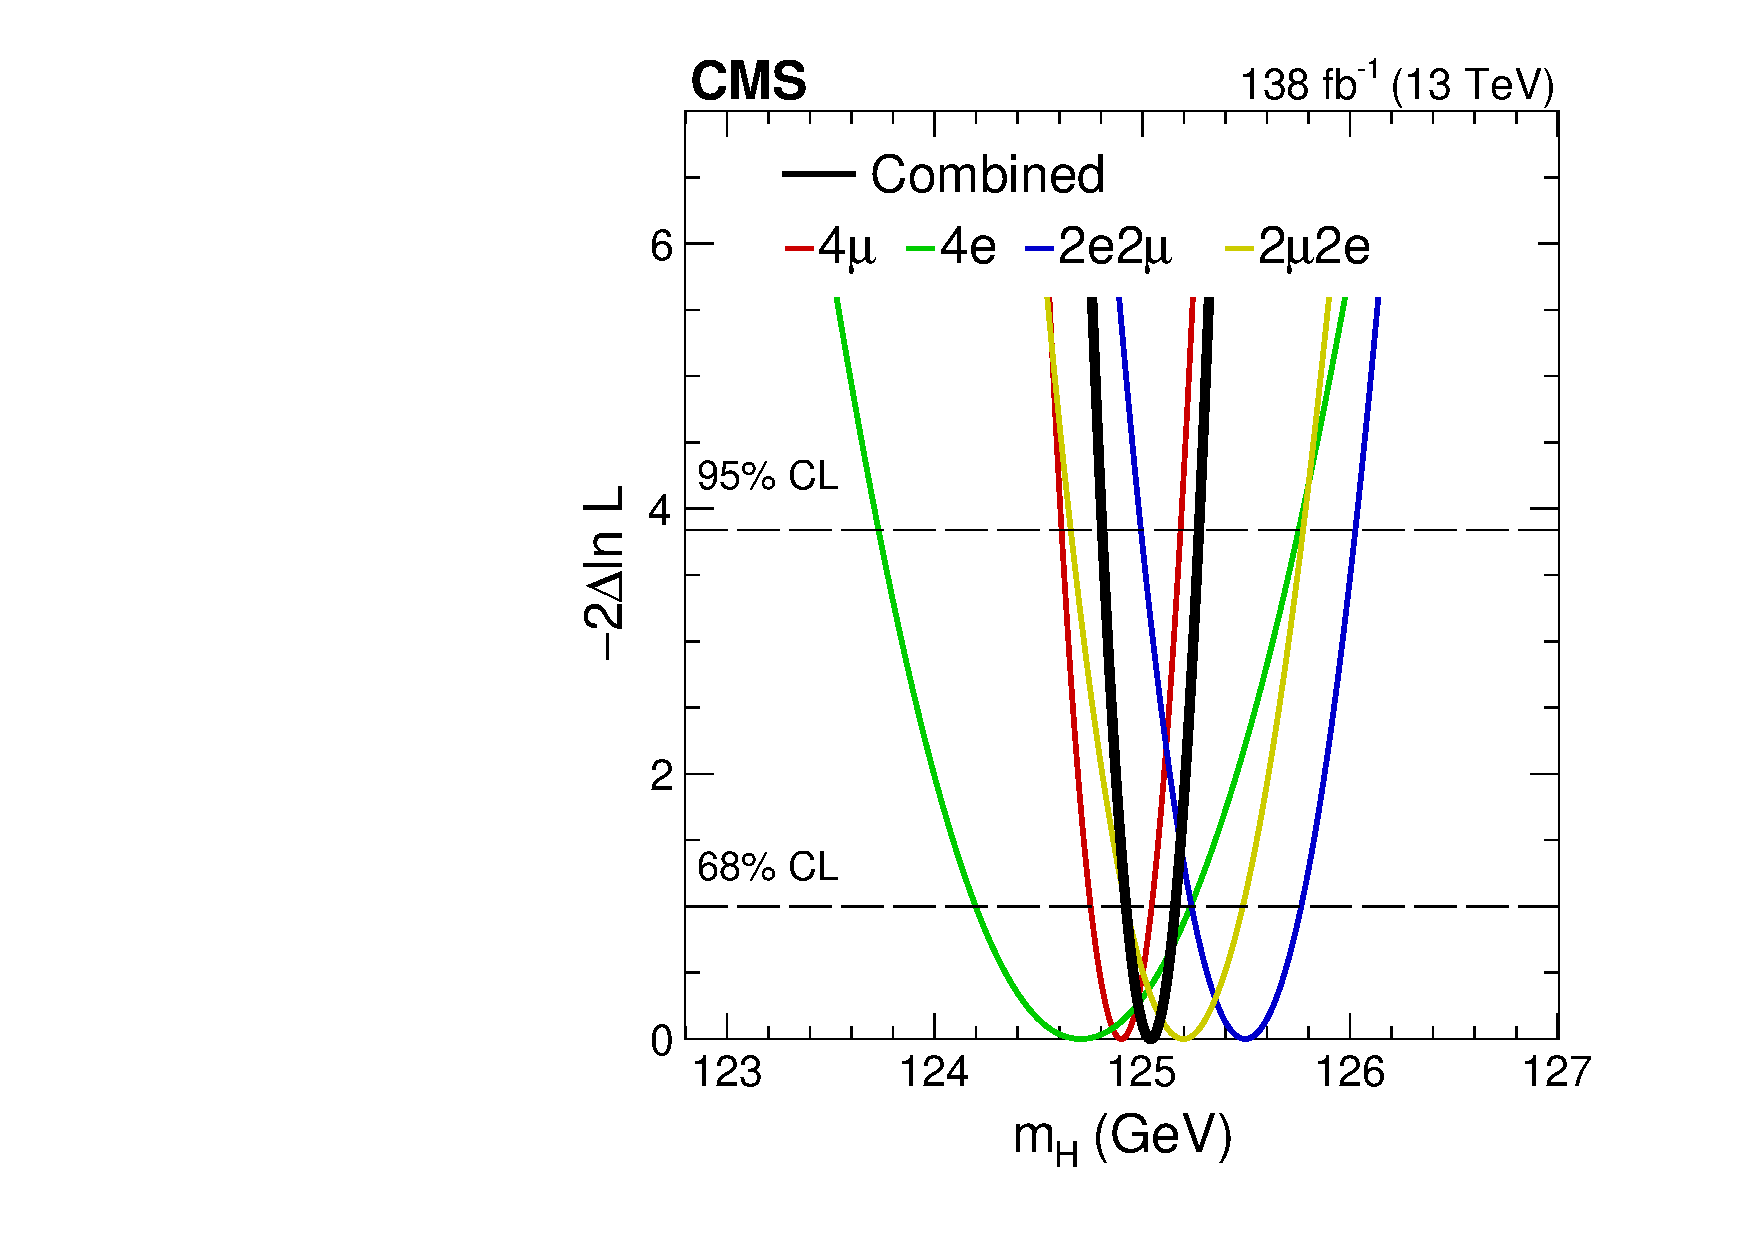
\includegraphics[width=0.45\textwidth]{Figure_008.pdf}
  \caption{The profile likelihood from the $m_H$ fit using the $\mathcal{N}$--2D$'_\text{BS}$ model for each of the 4$\ell$ categories and combined.  The change in likelihood corresponding to 68 and 95\% CLs are shown by the dashed horizontal lines. Both statistical and systematic uncertainties are included in the fits.}
  \label{MassLikelihoodScan}
\end{figure}

\begin{figure*}[!htb]
  \centering
  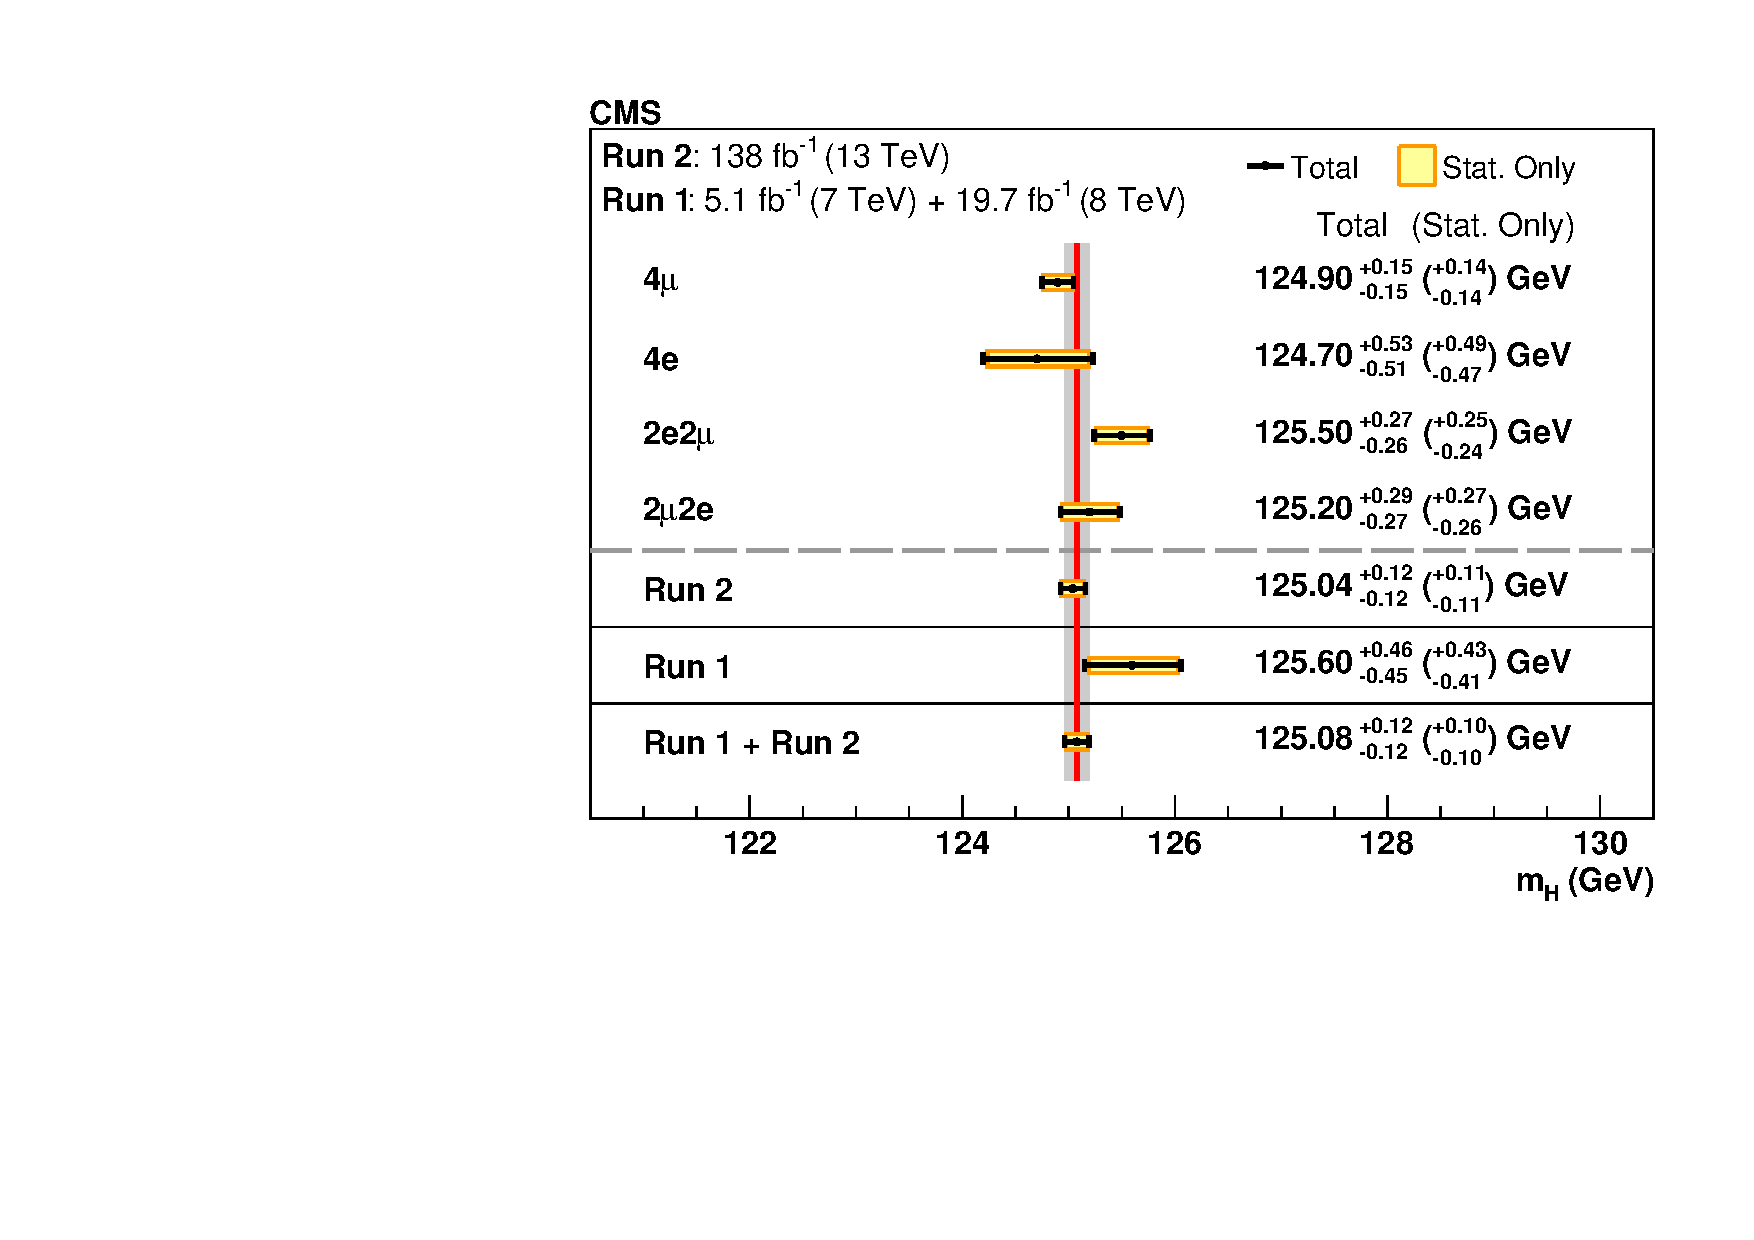
\includegraphics[width=0.60\textwidth]{Figure_009.pdf}
  \caption{Summary of the CMS Higgs boson mass measurements using the four-lepton final state. The red vertical line and the gray column represent the best fit value and the total uncertainty, respectively, as measured by combining the Runs 1 and 2 data. The yellow band and horizontal black bars show the statistical and total uncertainties in each measurement, respectively. The value of each measurement is given, along with the total and statistical only (in parentheses) uncertainties.}
  \label{Run1Run2_scan}
\end{figure*}
